\documentclass{beamer}
\usepackage{basileabeam}
\usepackage{graphicx}
\usepackage{subcaption}
\usepackage{animate,media9,movie15}
\usepackage{listings}

\usepackage[font=small,labelfont=bf]{caption}

%notes
%\pgfpagesuselayout{2 on 1}[a4paper,border shrink=5mm]
%\setbeamertemplate{note page}[plain]
%\setbeameroption{show notes on second screen=right}

\title              {Database Project}
\author             {Manuel Rickli, Lukas Stöckli}
\email				{manuel.rickli@unibas.ch, lukas.stoeckli@unibas.ch}
\institute          {University of Basel}

\date               {11.01.2019}

\ulogo        		{Template/header}
\ulistelement    	{Template/listelement}

\graphicspath{{../Output/}}

% I will give explanations of subjects as they appear (combination of Foundations, Data Set Analysis and Implementation)
%
% Motivation: what we want to find out, what would be the benefit
% Contribution: what have we done, how do we benefit from it
% data sets and implementation: short overview of the data sources and noteworthy parts of the implementation;

\begin{document}
\begin{frame}[t,plain]
	\titlepage
\end{frame}

\note{Bachelor's thesis presentation}

% CONTENT
\begin{frame}
	\begin{tabularx}{\textwidth}{X}
		\hline
		\rowcolor{hcolor}
		Datasets \& Schema\\
		\hline
		Analysis Goals\\
		\hline
		Results\\
		\hline
	\end{tabularx}
\end{frame}


% DATASETS
\begin{frame}{Datasets:}
	\begin{itemize}
		\item Global Terrorism 1970 - 2017
		\begin{itemize}
			\item Dimensions: 181'691 rows x 135 columns
			\item Size: 162.8 MB
		\end{itemize}
		\item Metal bands 1964 - 2016
		\begin{itemize}
			\item Dimensions: 5000 rows x 7 columns
			\item Size: 264 KB
		\end{itemize}
		\item World Population 1960 - 2015
		\begin{itemize}
			\item Dimensions: 264 rows x 57 columns
			\item Size: 125 KB
		\end{itemize}
		\item Weather Data
		\begin{itemize}
			\item Inventory
			\begin{itemize}
			  \item Dimensions: 65236 rows x 6 columns
			  \item Size: 26.9 MB
		    \end{itemize}
			\item Daily
			\begin{itemize}
			  \item Dimensions: $\sim$10M rows x 35 columns
			  \item Size: 2.9 GB
		    \end{itemize}
		\end{itemize}
	\end{itemize}
\end{frame}


% SINGLE SOURCES
\begin{frame}{Single sources}
	\begin{figure}
		\begin{subfigure}[b]{0.315\textwidth}
			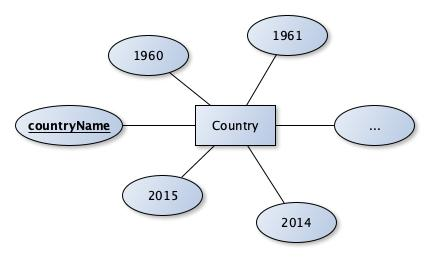
\includegraphics[width=\textwidth]{ER/g2-country.jpg}
		\end{subfigure}
		\begin{subfigure}[b]{0.315\textwidth}
			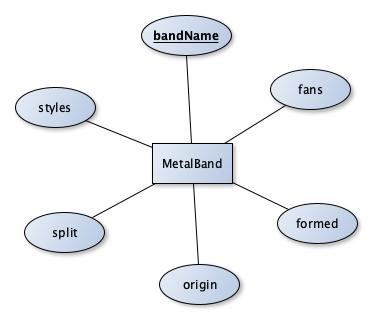
\includegraphics[width=\textwidth]{ER/g2-metal.jpg}
		\end{subfigure}
		\begin{subfigure}[b]{0.315\textwidth}
			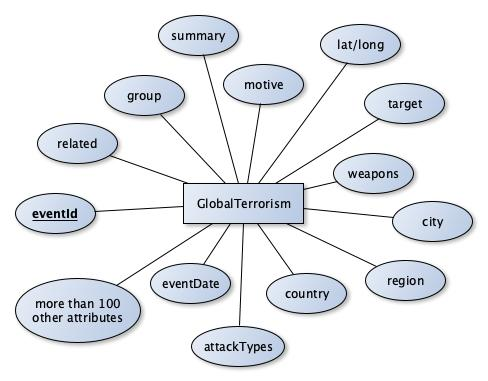
\includegraphics[width=\textwidth]{ER/g2-terror.jpg}
		\end{subfigure}
	\end{figure}
	\begin{figure}
		\begin{subfigure}[b]{0.7\textwidth}
			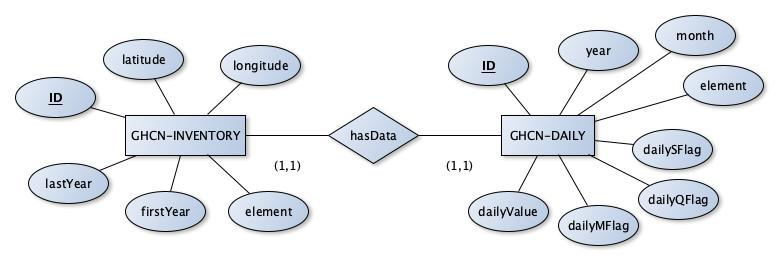
\includegraphics[width=\textwidth]{ER/g2-weather.jpg}
		\end{subfigure}
	\end{figure}
\end{frame}


% INTEGRATED SCHEMA
\begin{frame}{Integrated schema}
	\begin{figure}
		\begin{subfigure}[b]{\textwidth}
			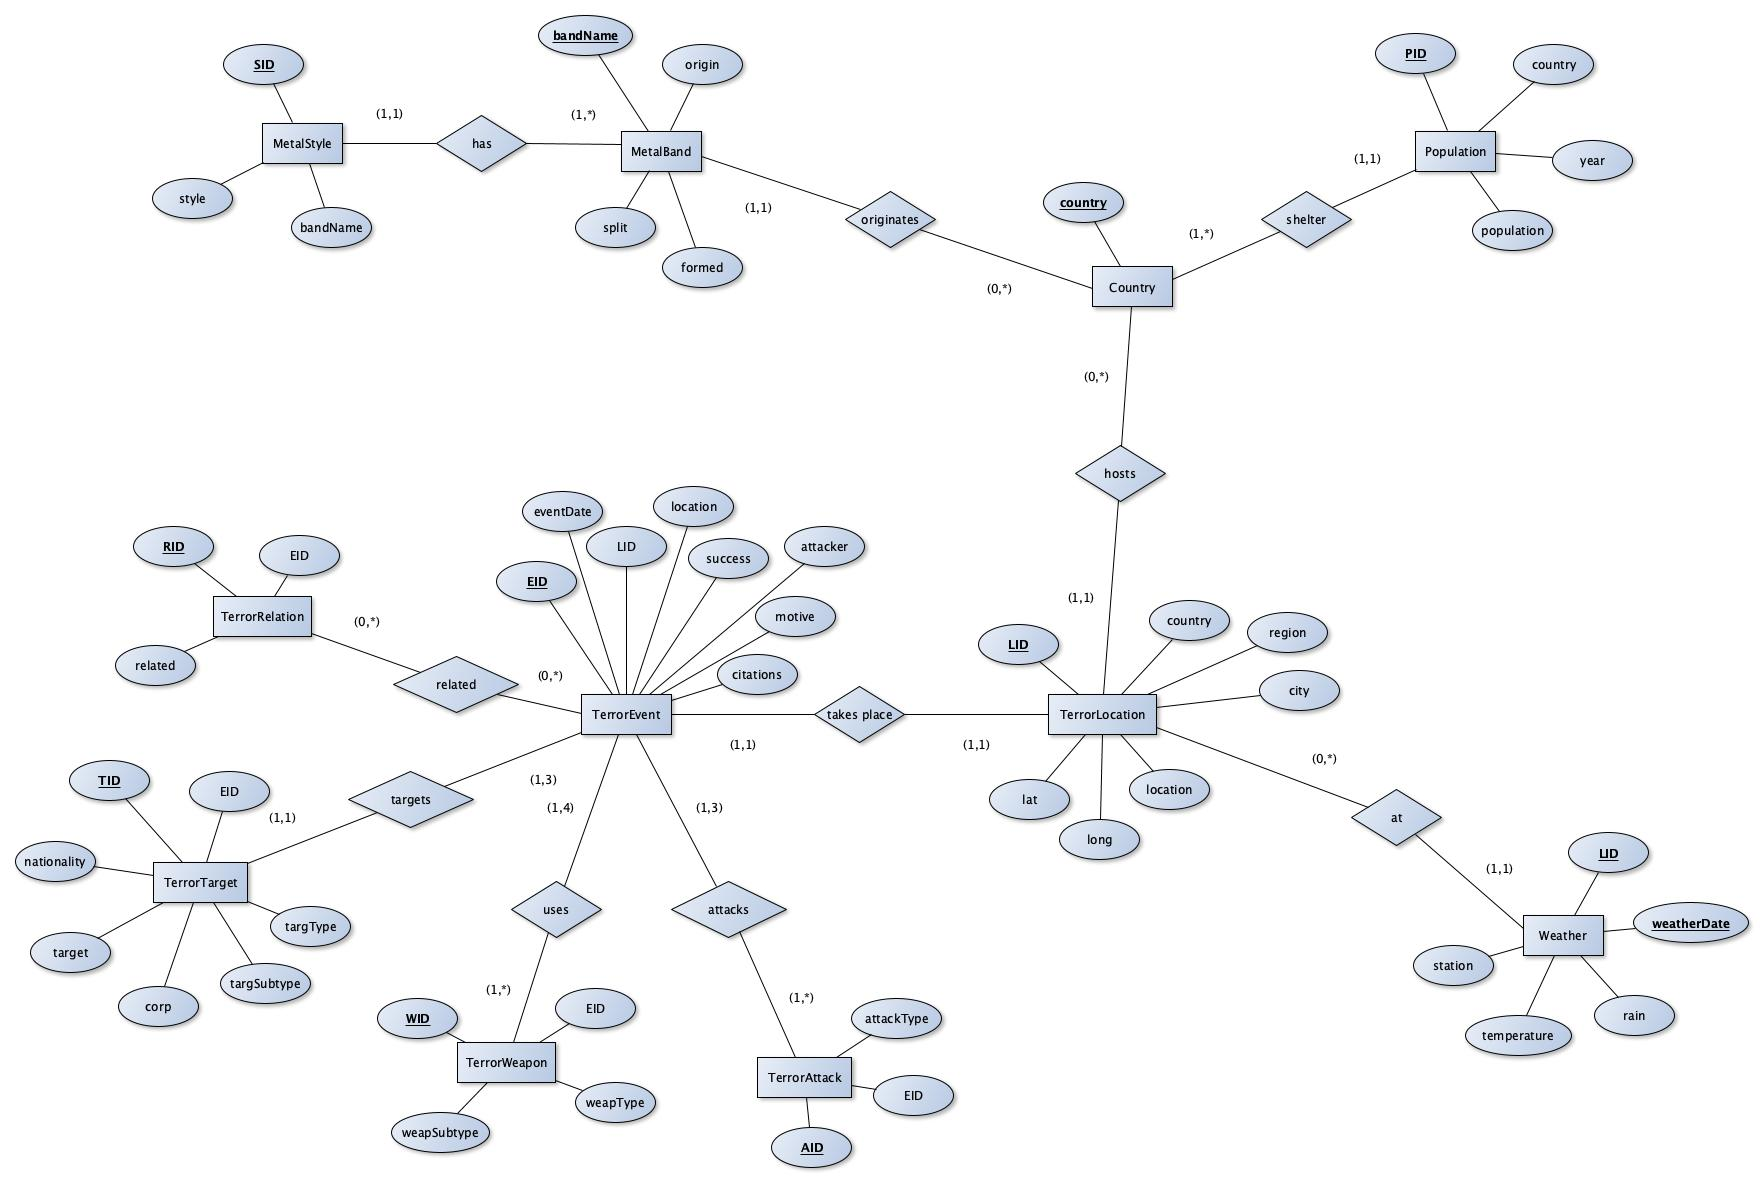
\includegraphics[width=\textwidth]{ER/g2-integratedSchema.jpg}
		\end{subfigure}
	\end{figure}
\end{frame}


% CONTENT
\begin{frame}
	\begin{tabularx}{\textwidth}{X}
		\hline
		Datasets \& Schema\\
		\hline
		\rowcolor{hcolor}
		Analysis Goals\\
		\hline
		Results\\
		\hline
	\end{tabularx}
\end{frame}


% ANALYSIS GOALS
\begin{frame}{Analysis goals}
	\begin{itemize}
		\item Are terror events dependent on the weather?
		\item Do terror attacks influence founding/splitting of metal bands and vice versa?
		\item Does the population influence the number of existing metal bands?
		\item Do terror attacks have an influence on the population?
		\item Which main genre has the most terror events?
	\end{itemize}
\end{frame}


% CONTENT
\begin{frame}
	\begin{tabularx}{\textwidth}{X}
		\hline
		Datasets \& Schema\\
		\hline
		Analysis Goals\\
		\hline
		\rowcolor{hcolor}
		Results\\
		\hline
	\end{tabularx}
\end{frame}

\begin{frame}{Results}
	Attack Types
	
	\begin{figure}
		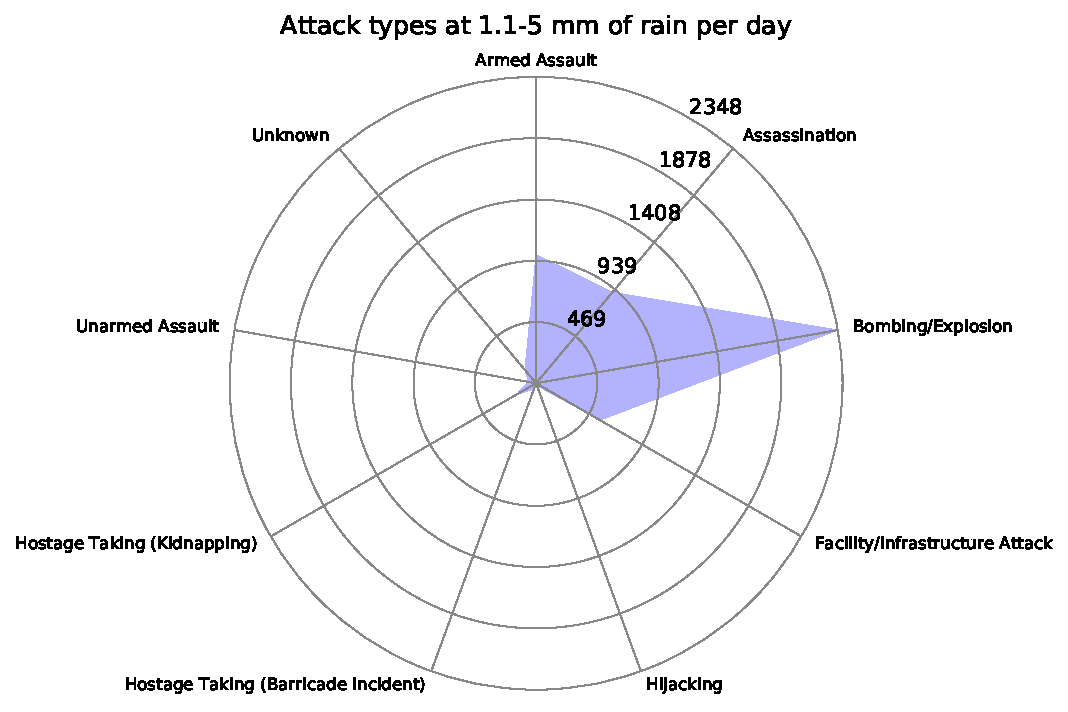
\includegraphics[width=0.8\textwidth]{Rain-Attack/rain11-5_starDiagram}
	\end{figure}
	
\end{frame}

\begin{frame}{Results}
	\begin{itemize}
		\item 
		Are terror attacks dependent on the weather?
		\begin{itemize}
			\item Attack types - Rain
		\end{itemize}
	\end{itemize}
	
	\begin{figure}
		\begin{subfigure}[b]{0.3\textwidth}
			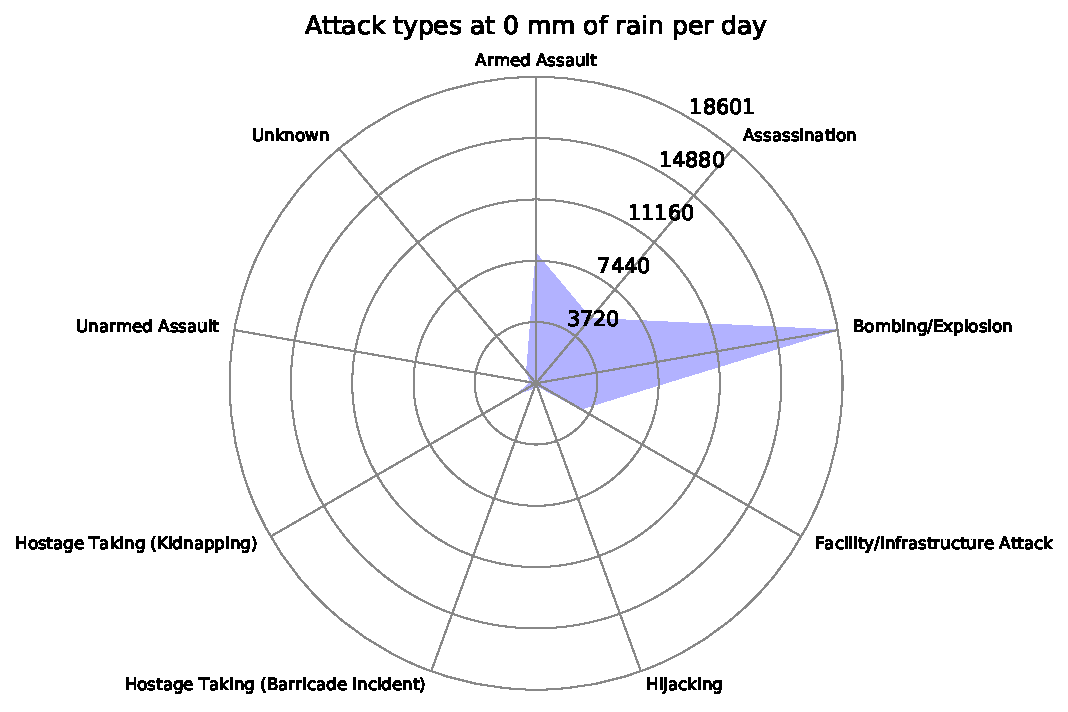
\includegraphics[width=\textwidth]{Rain-Attack/rain0_starDiagram}
		\end{subfigure}
		\begin{subfigure}[b]{0.3\textwidth}
			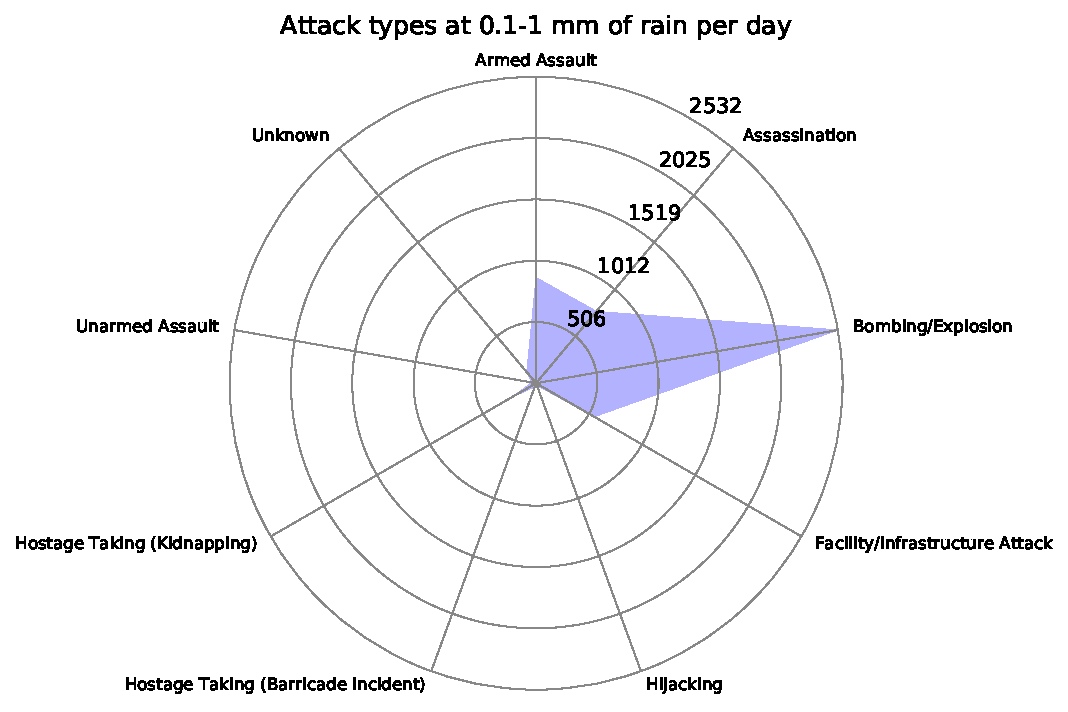
\includegraphics[width=\textwidth]{Rain-Attack/rain01-1_starDiagram}
		\end{subfigure}
		\begin{subfigure}[b]{0.3\textwidth}
			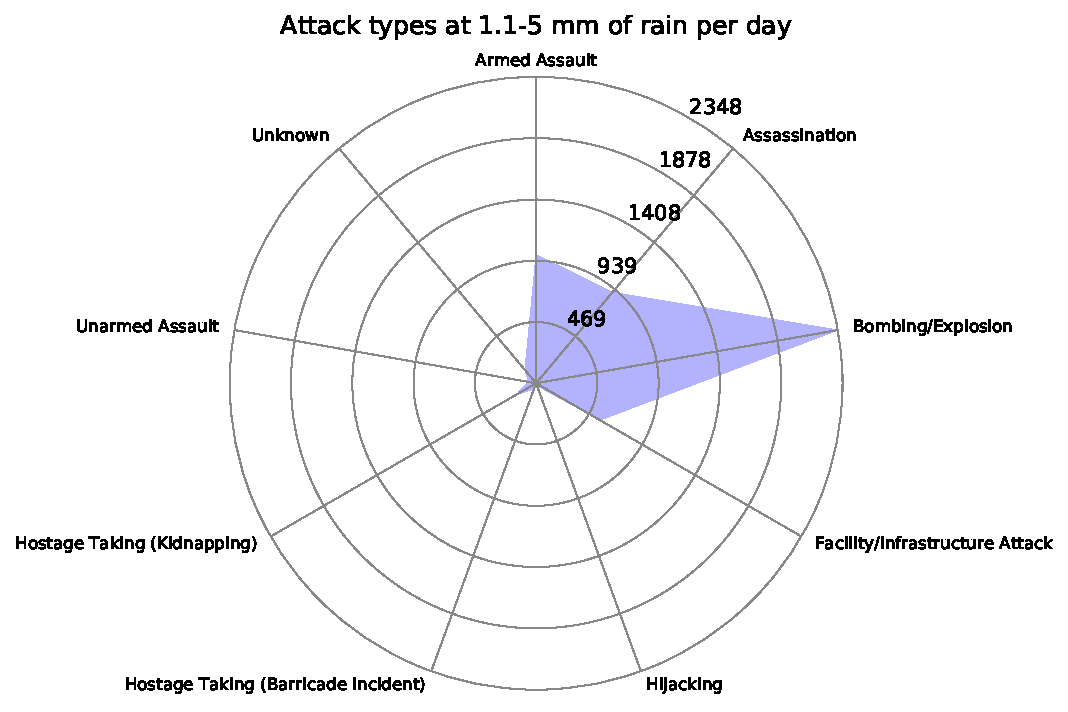
\includegraphics[width=\textwidth]{Rain-Attack/rain11-5_starDiagram}
		\end{subfigure}
	\end{figure}
	\begin{figure}
		\begin{subfigure}[b]{0.3\textwidth}
			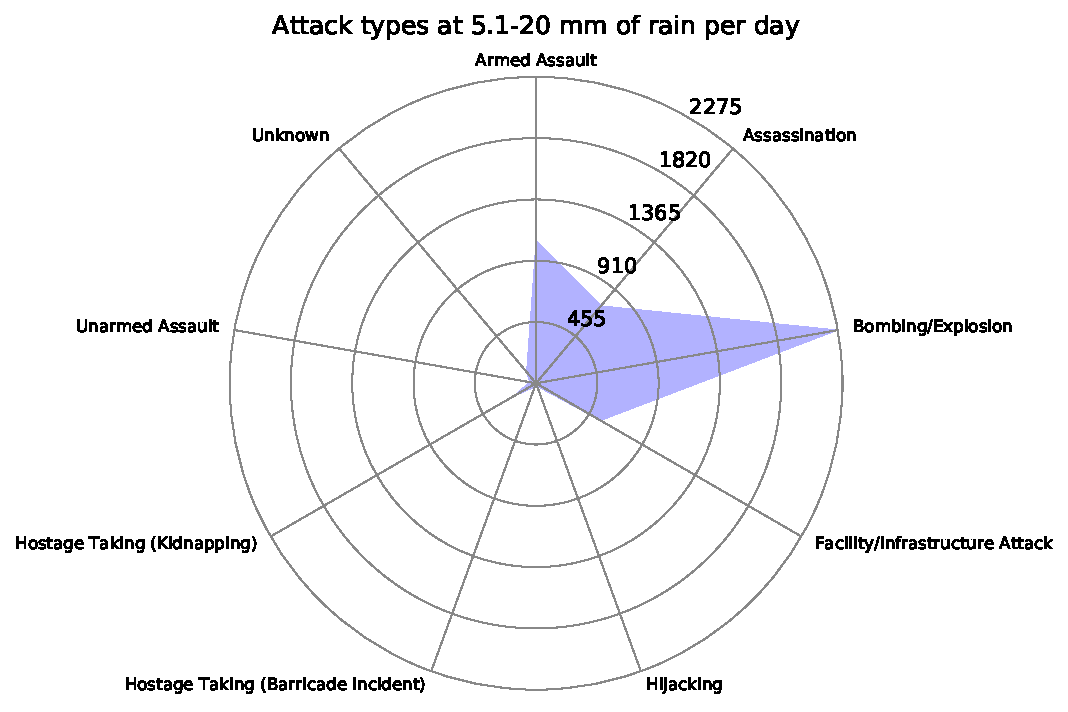
\includegraphics[width=\textwidth]{Rain-Attack/rain51-20_starDiagram}
		\end{subfigure}
		\begin{subfigure}[b]{0.3\textwidth}
			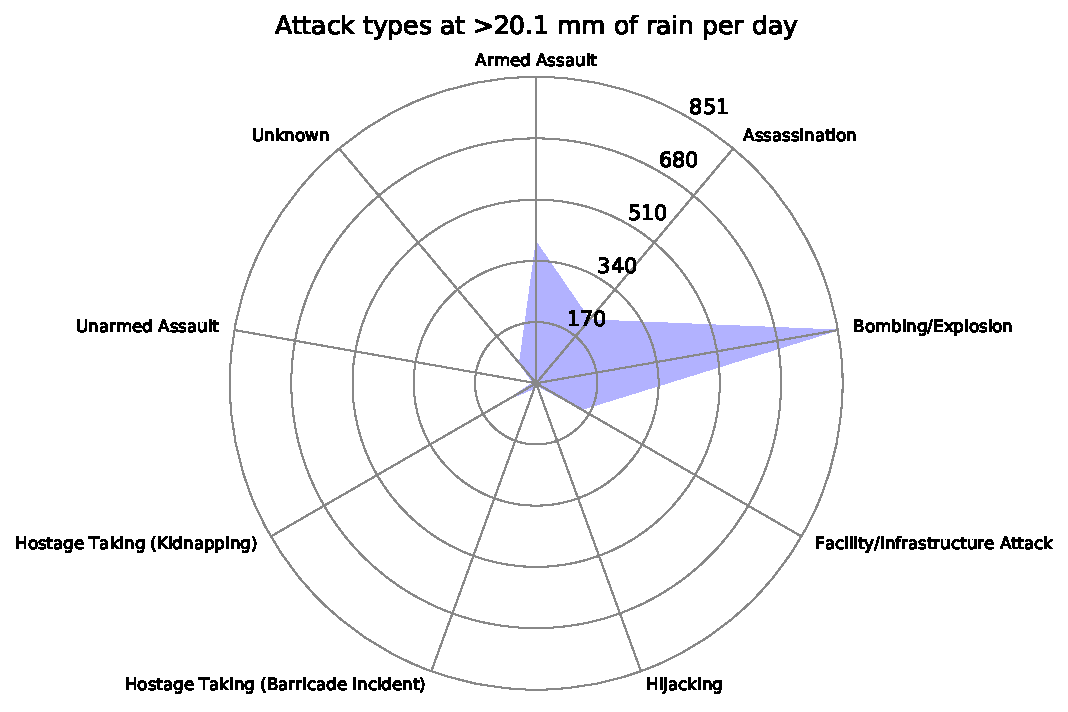
\includegraphics[width=\textwidth]{Rain-Attack/rain>201_starDiagram}
		\end{subfigure}
	\end{figure}
	
\end{frame}

\begin{frame}{Results}
	\begin{itemize}
		\item 
		Are terror attacks dependent on the weather?
		\begin{itemize}
			\item Attack types - Temperature
		\end{itemize}
	\end{itemize}
	
	\begin{figure}

		\begin{subfigure}[b]{0.3\textwidth}
			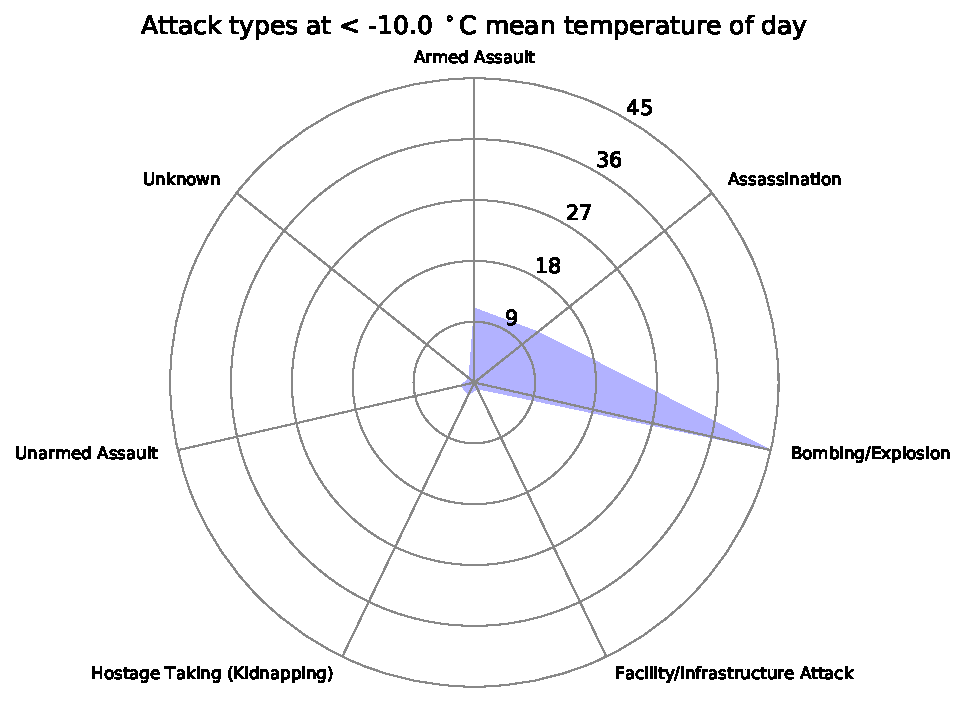
\includegraphics[width=\textwidth]{Temp-Attack/temp<-100_starDiagram}
		\end{subfigure}
		\begin{subfigure}[b]{0.3\textwidth}
			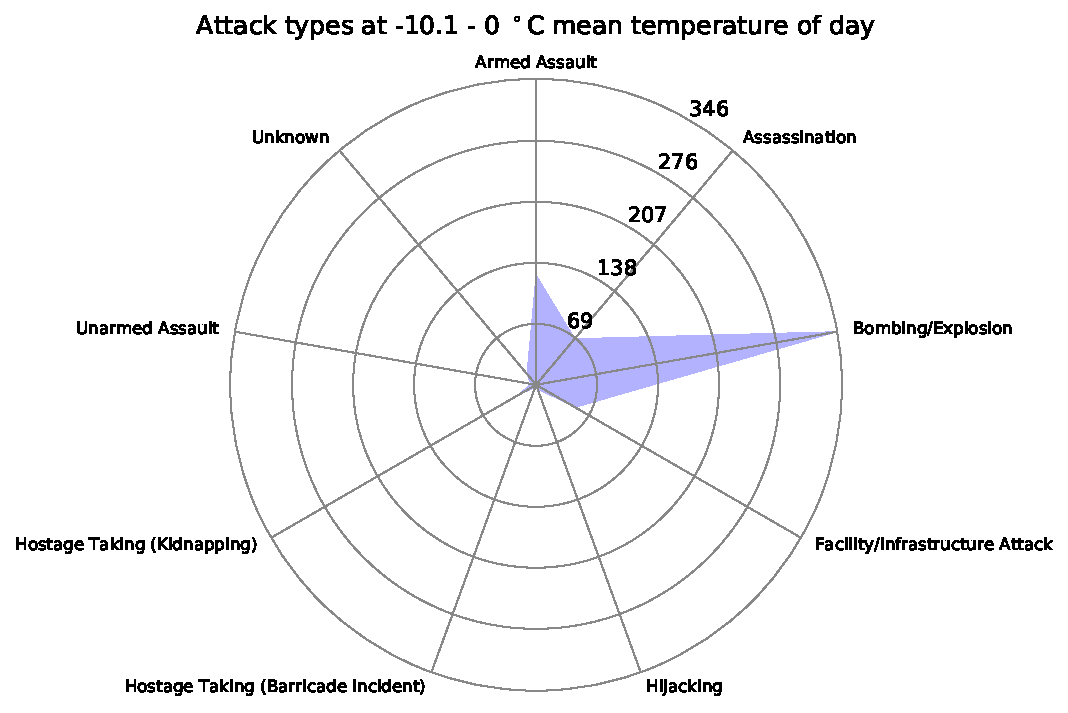
\includegraphics[width=\textwidth]{Temp-Attack/temp-101-0_starDiagram}
		\end{subfigure}
		\begin{subfigure}[b]{0.3\textwidth}
			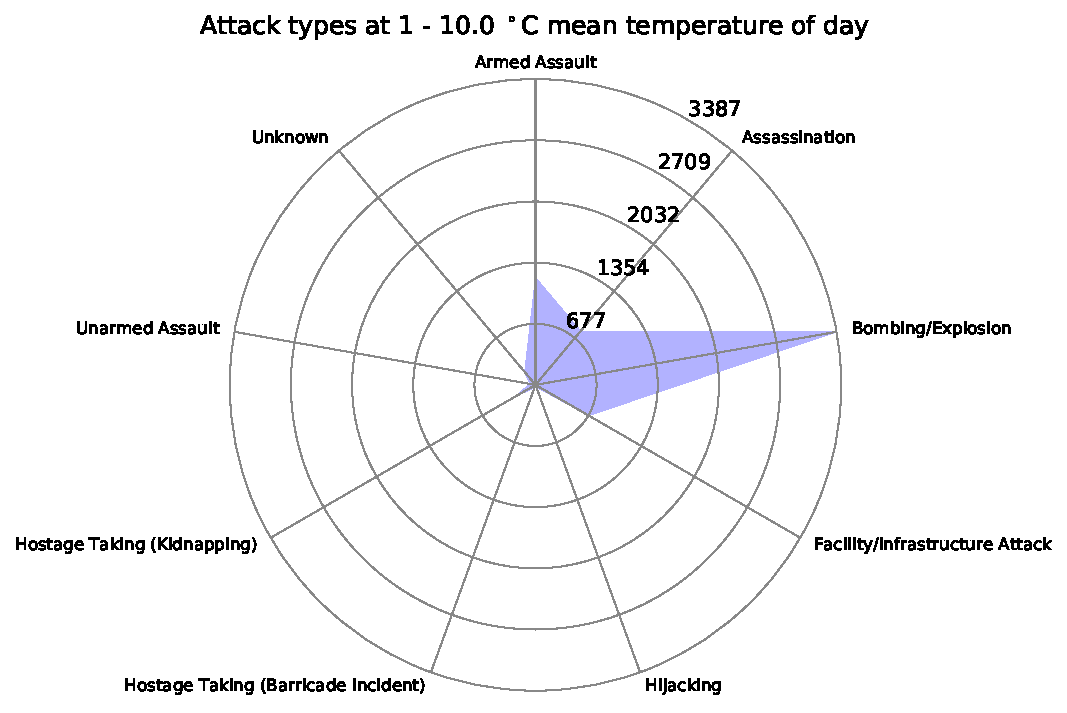
\includegraphics[width=\textwidth]{Temp-Attack/temp1-100_starDiagram}
		\end{subfigure}
	\end{figure}
	\begin{figure}
		\begin{subfigure}[b]{0.3\textwidth}
			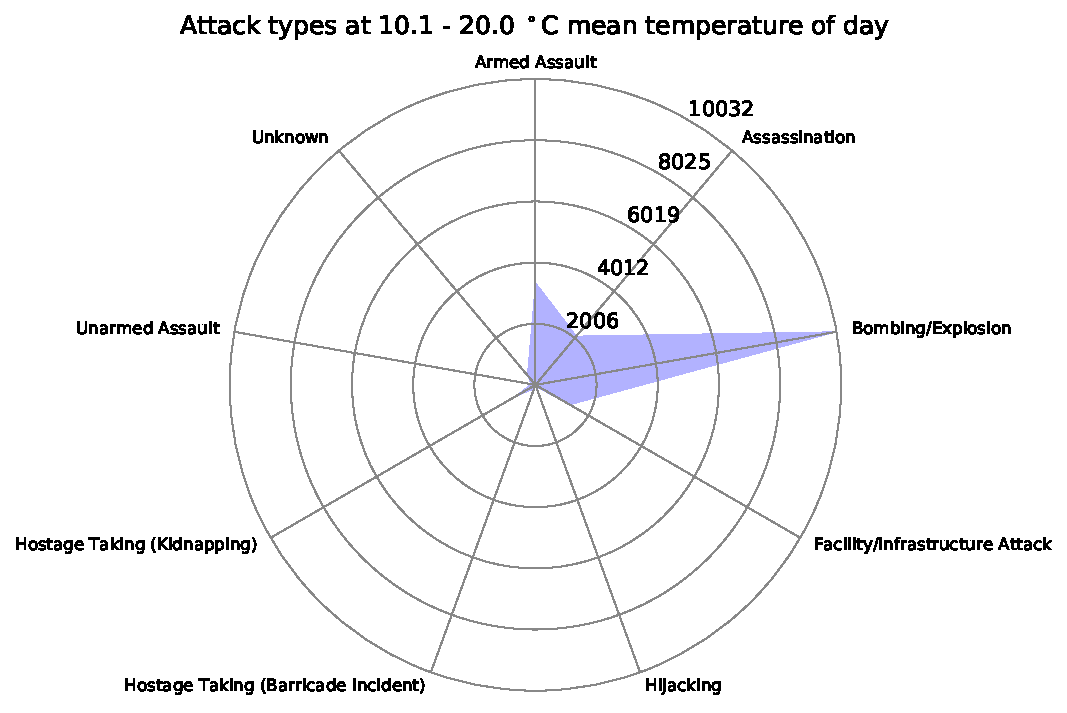
\includegraphics[width=\textwidth]{Temp-Attack/temp101-200_starDiagram}
		\end{subfigure}
		\begin{subfigure}[b]{0.3\textwidth}
			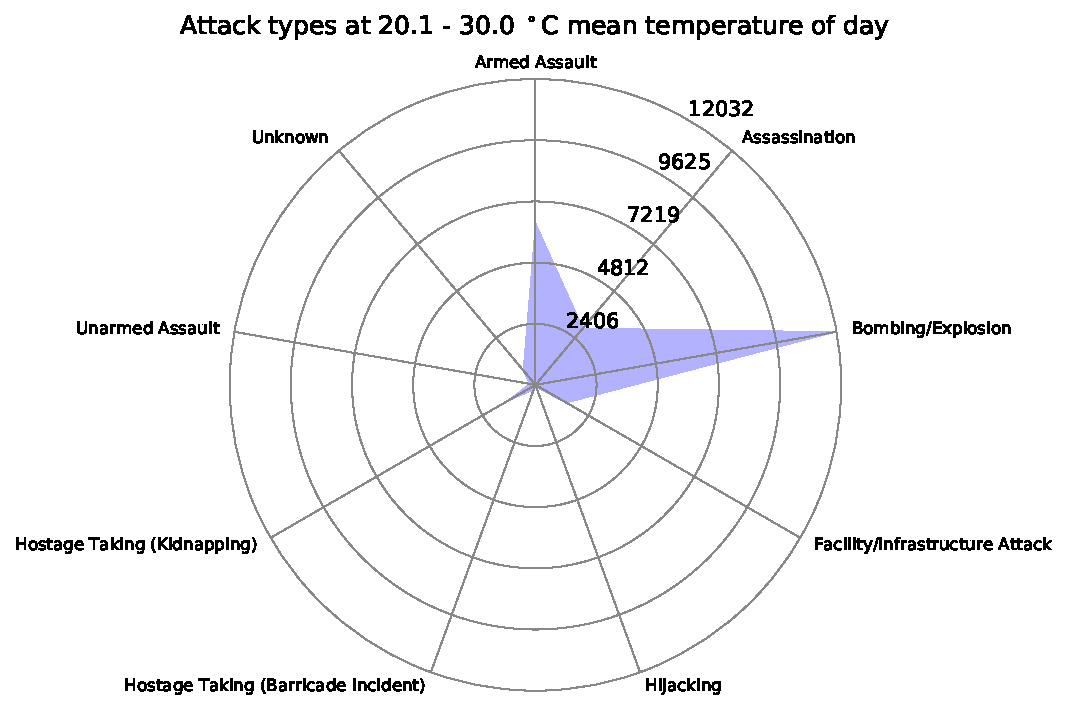
\includegraphics[width=\textwidth]{Temp-Attack/temp201-300_starDiagram}
		\end{subfigure}
		\begin{subfigure}[b]{0.3\textwidth}
			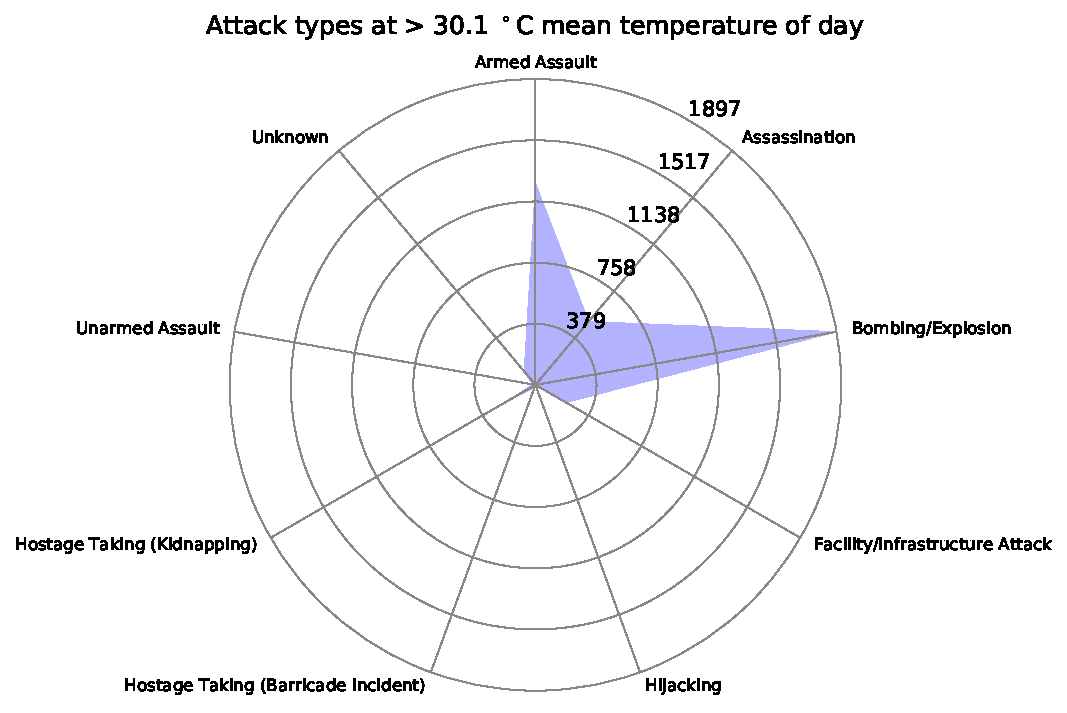
\includegraphics[width=\textwidth]{Temp-Attack/temp>301_starDiagram}
		\end{subfigure}
	\end{figure}
	
\end{frame}

\begin{frame}{Results}
	Attack Targets
	
	\begin{figure}
		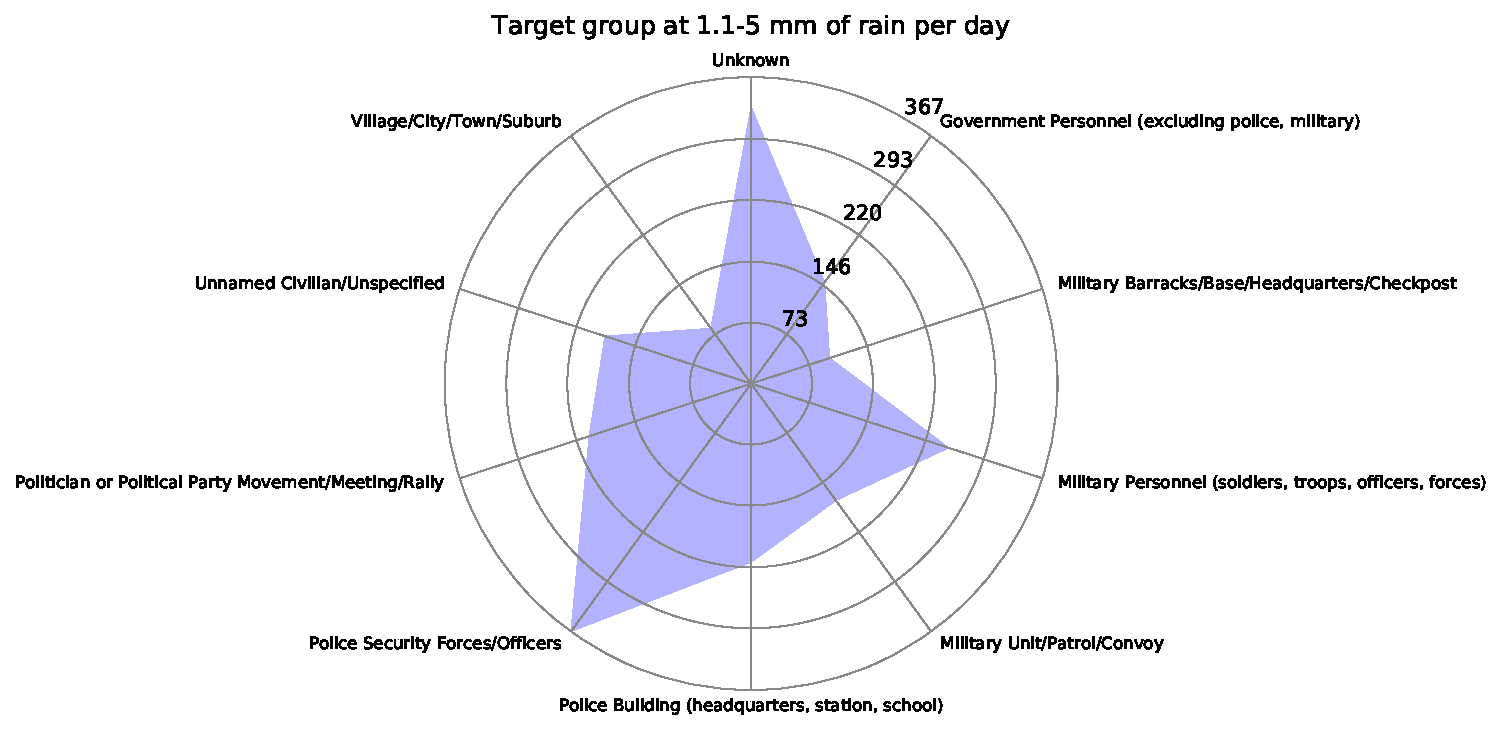
\includegraphics[width=\textwidth]{Rain-Target/rain11-5_starDiagram}
	\end{figure}
	
\end{frame}

\begin{frame}{Results}
	\begin{itemize}
		\item 
		Are attack targets dependent on the weather?
		\begin{itemize}
			\item Attack targets - Rain
		\end{itemize}
	\end{itemize}
	
	\begin{figure}
		\begin{subfigure}[b]{0.3\textwidth}
			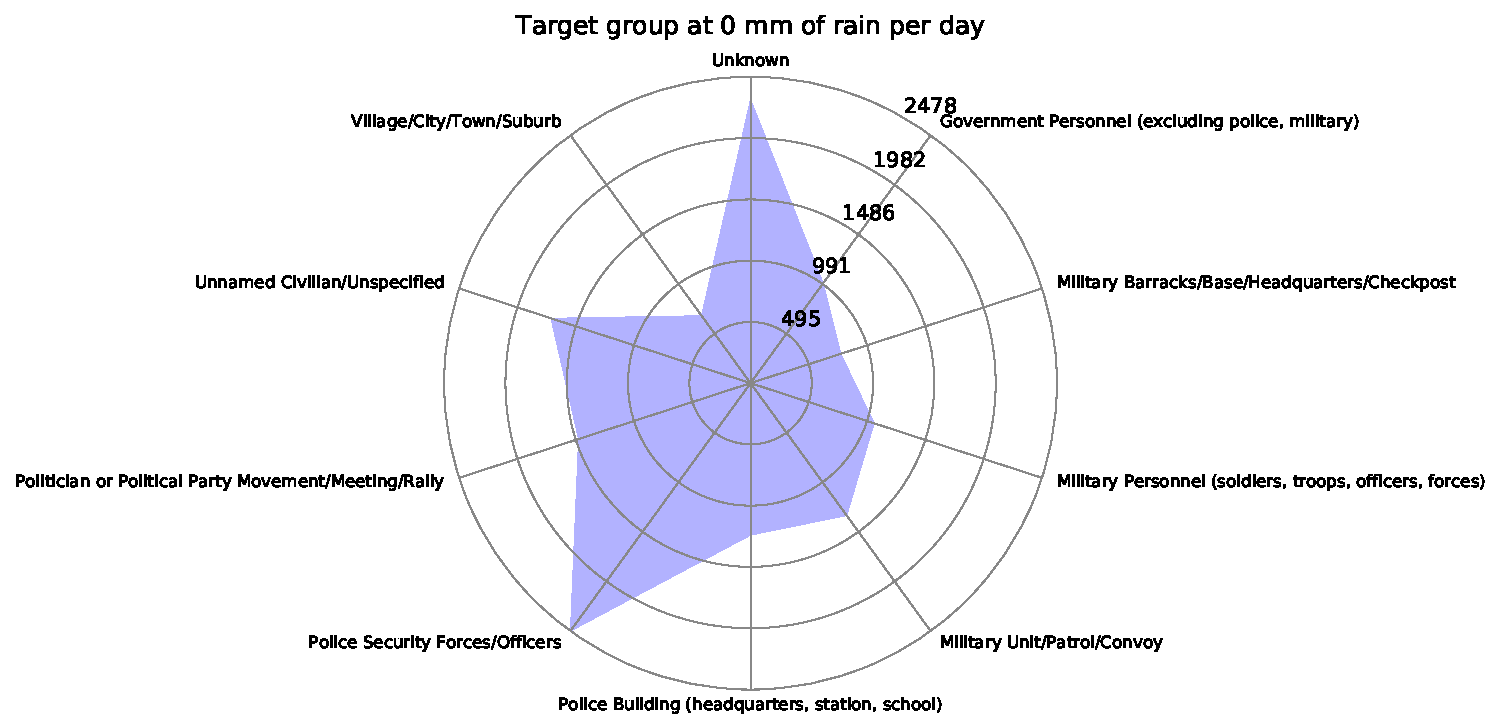
\includegraphics[width=\textwidth]{Rain-Target/rain0_starDiagram}
		\end{subfigure}
		\begin{subfigure}[b]{0.3\textwidth}
			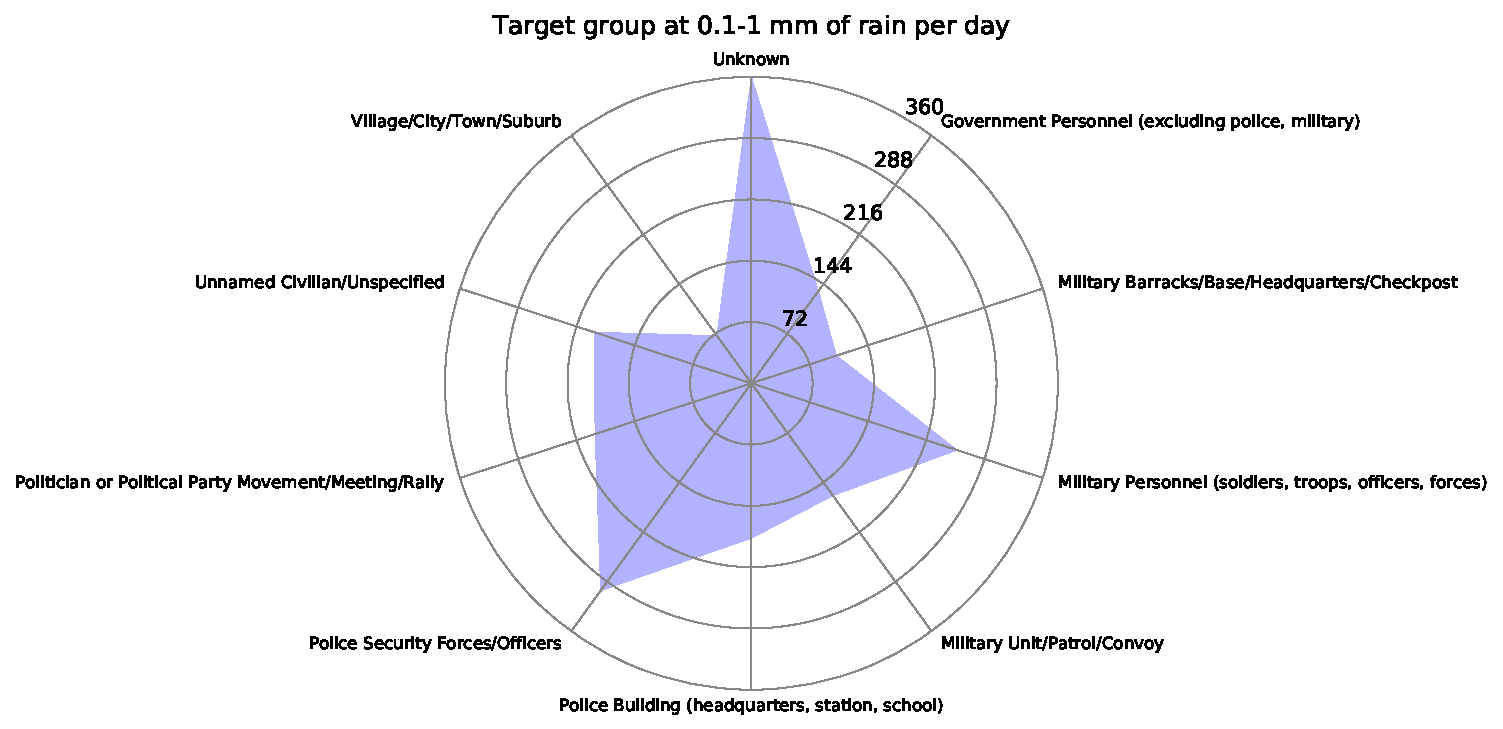
\includegraphics[width=\textwidth]{Rain-Target/rain01-1_starDiagram}
		\end{subfigure}
		\begin{subfigure}[b]{0.3\textwidth}
			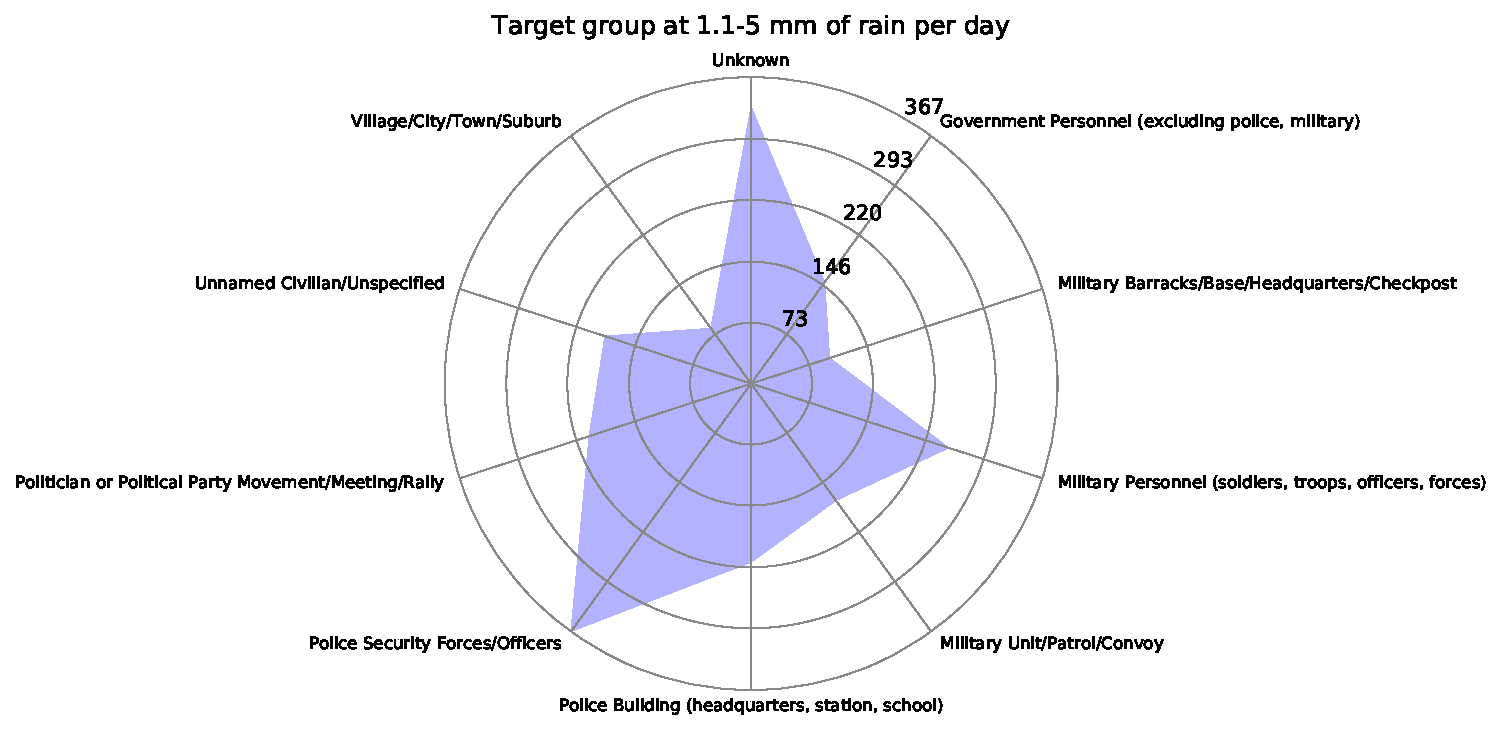
\includegraphics[width=\textwidth]{Rain-Target/rain11-5_starDiagram}
		\end{subfigure}
	\end{figure}
	\begin{figure}
		\begin{subfigure}[b]{0.3\textwidth}
			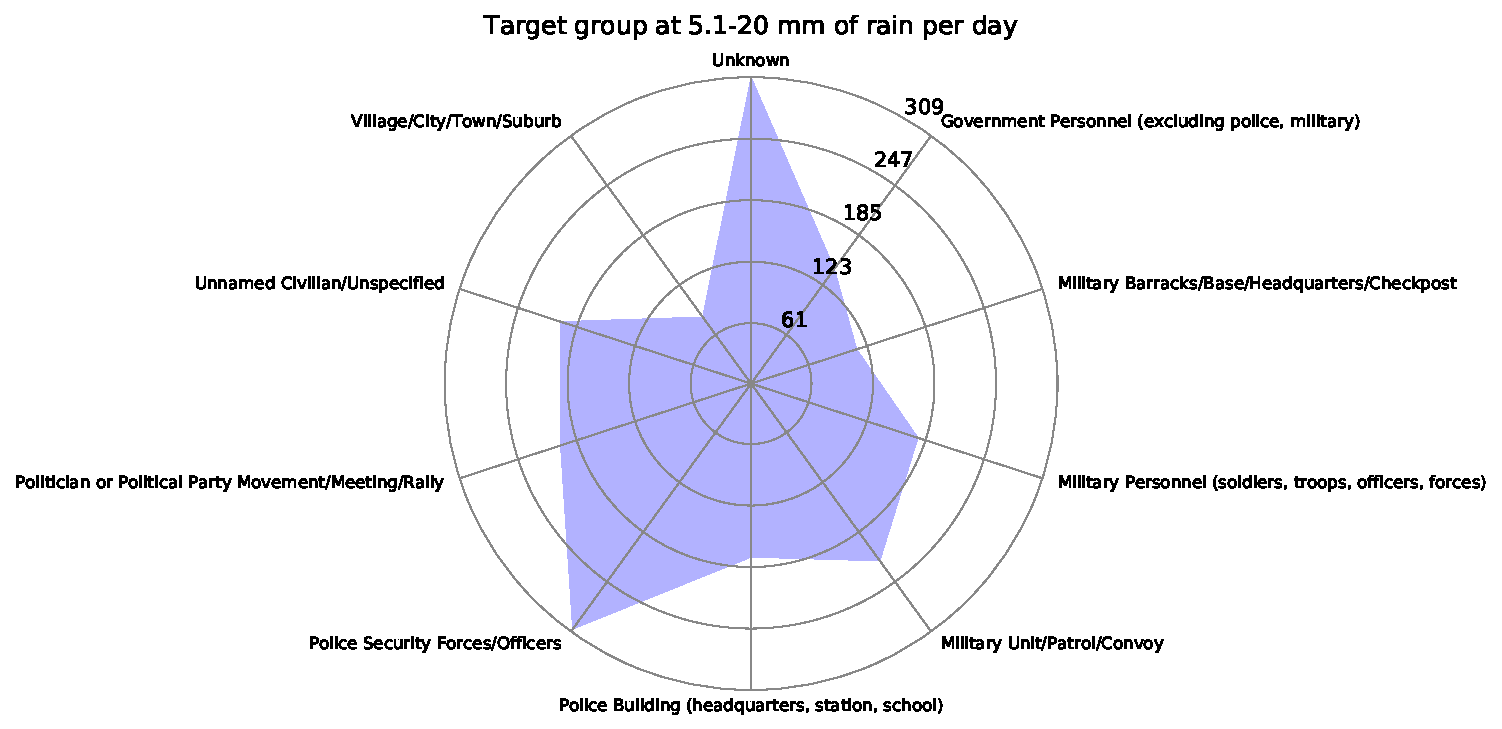
\includegraphics[width=\textwidth]{Rain-Target/rain51-20_starDiagram}
		\end{subfigure}
		\begin{subfigure}[b]{0.3\textwidth}
			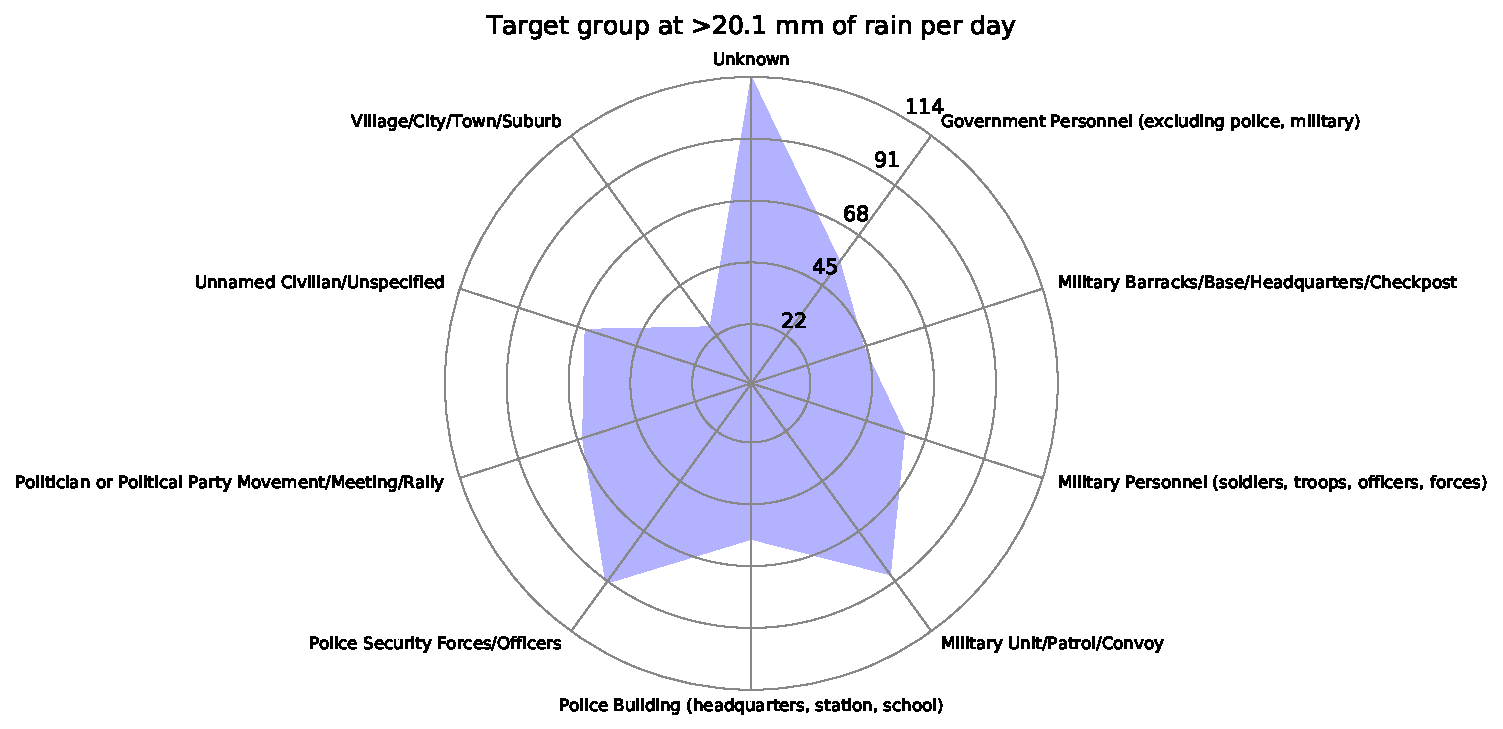
\includegraphics[width=\textwidth]{Rain-Target/rain>201_starDiagram}
		\end{subfigure}
	\end{figure}
	
\end{frame}

\begin{frame}{Results}
	\begin{itemize}
		\item 
		Are attack targets dependent on the weather?
		\begin{itemize}
			\item Attack targets - Temperature
		\end{itemize}
	\end{itemize}
	
	\begin{figure}

		\begin{subfigure}[b]{0.3\textwidth}
			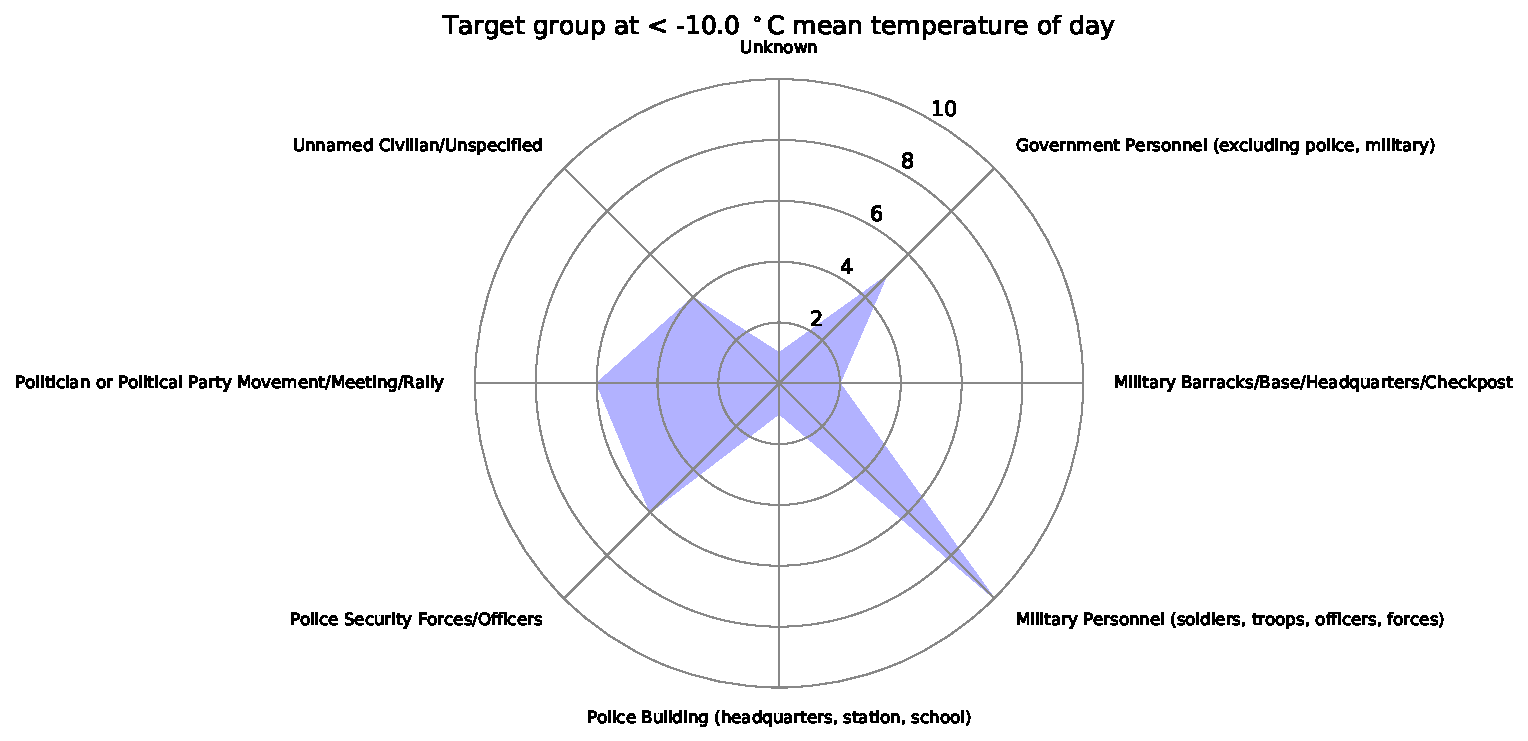
\includegraphics[width=\textwidth]{Temp-Target/temp<-100_starDiagram}
		\end{subfigure}
		\begin{subfigure}[b]{0.3\textwidth}
			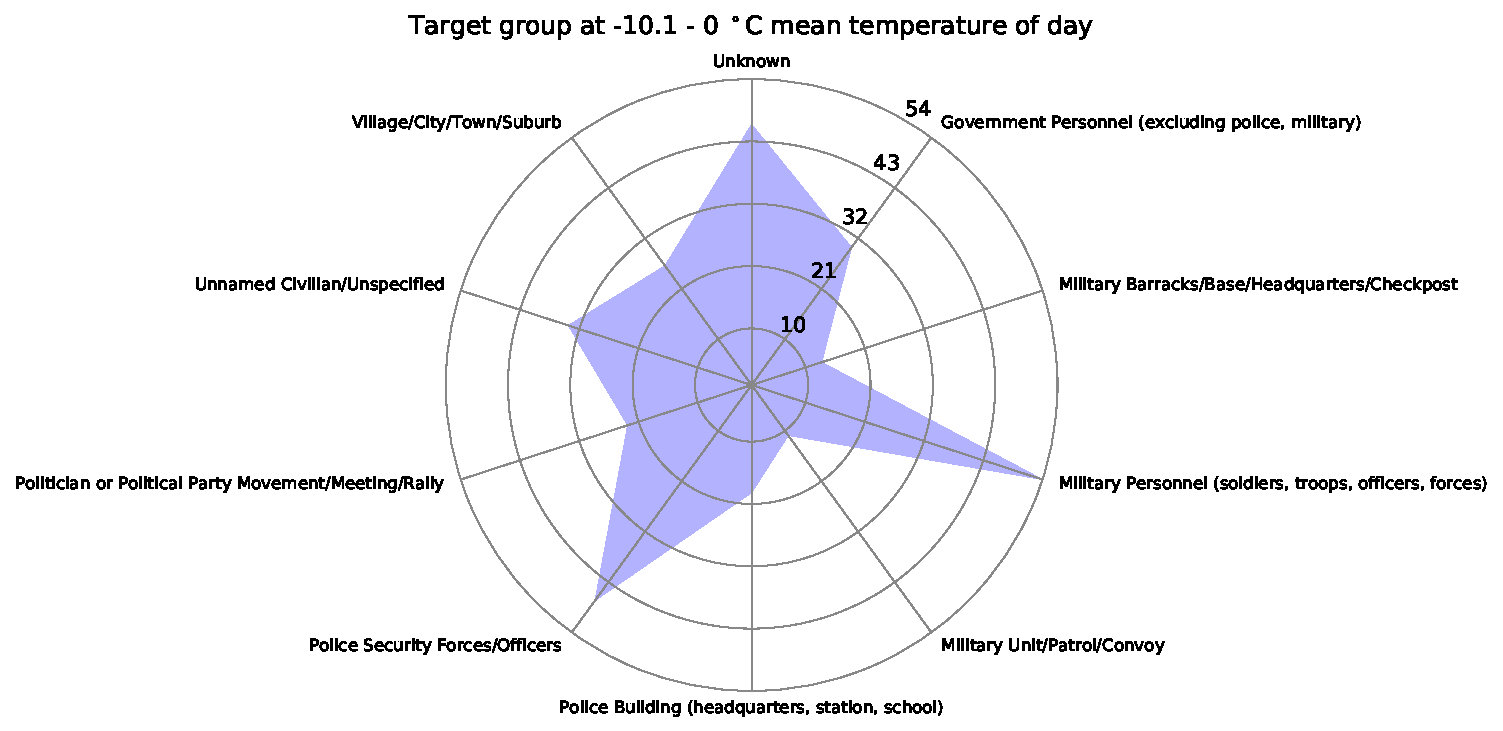
\includegraphics[width=\textwidth]{Temp-Target/temp-101-0_starDiagram}
		\end{subfigure}
		\begin{subfigure}[b]{0.3\textwidth}
			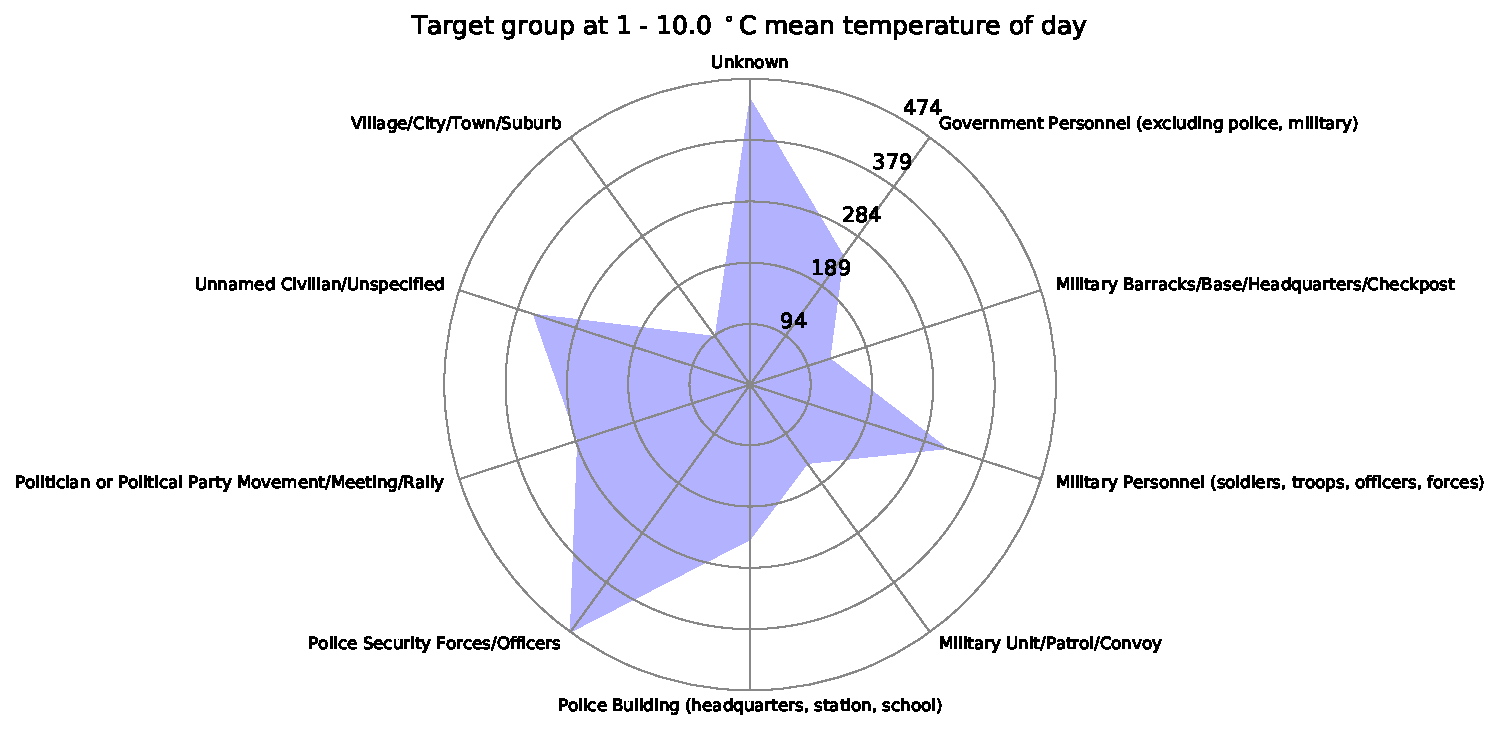
\includegraphics[width=\textwidth]{Temp-Target/temp1-100_starDiagram}
		\end{subfigure}
	\end{figure}
	\begin{figure}
		\begin{subfigure}[b]{0.3\textwidth}
			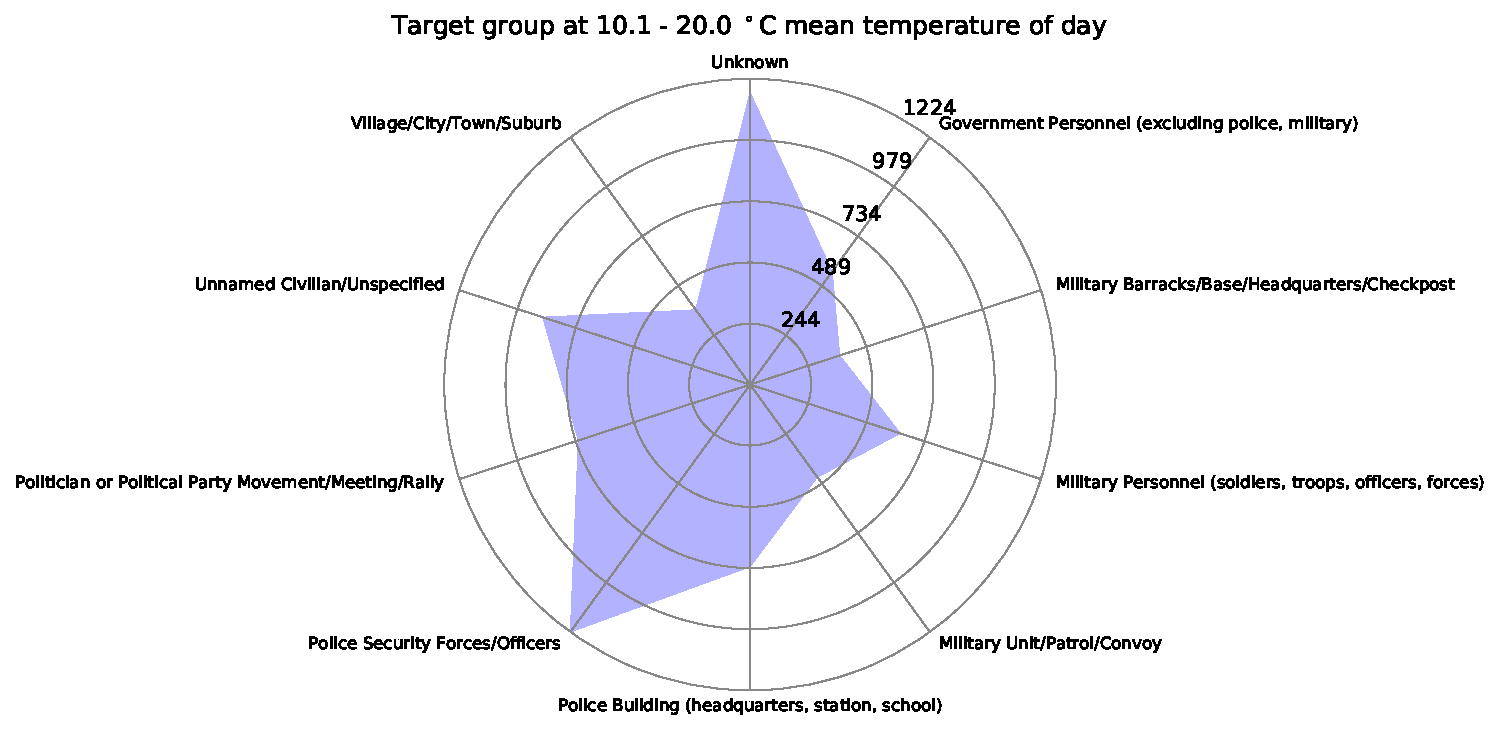
\includegraphics[width=\textwidth]{Temp-Target/temp101-200_starDiagram}
		\end{subfigure}
		\begin{subfigure}[b]{0.3\textwidth}
			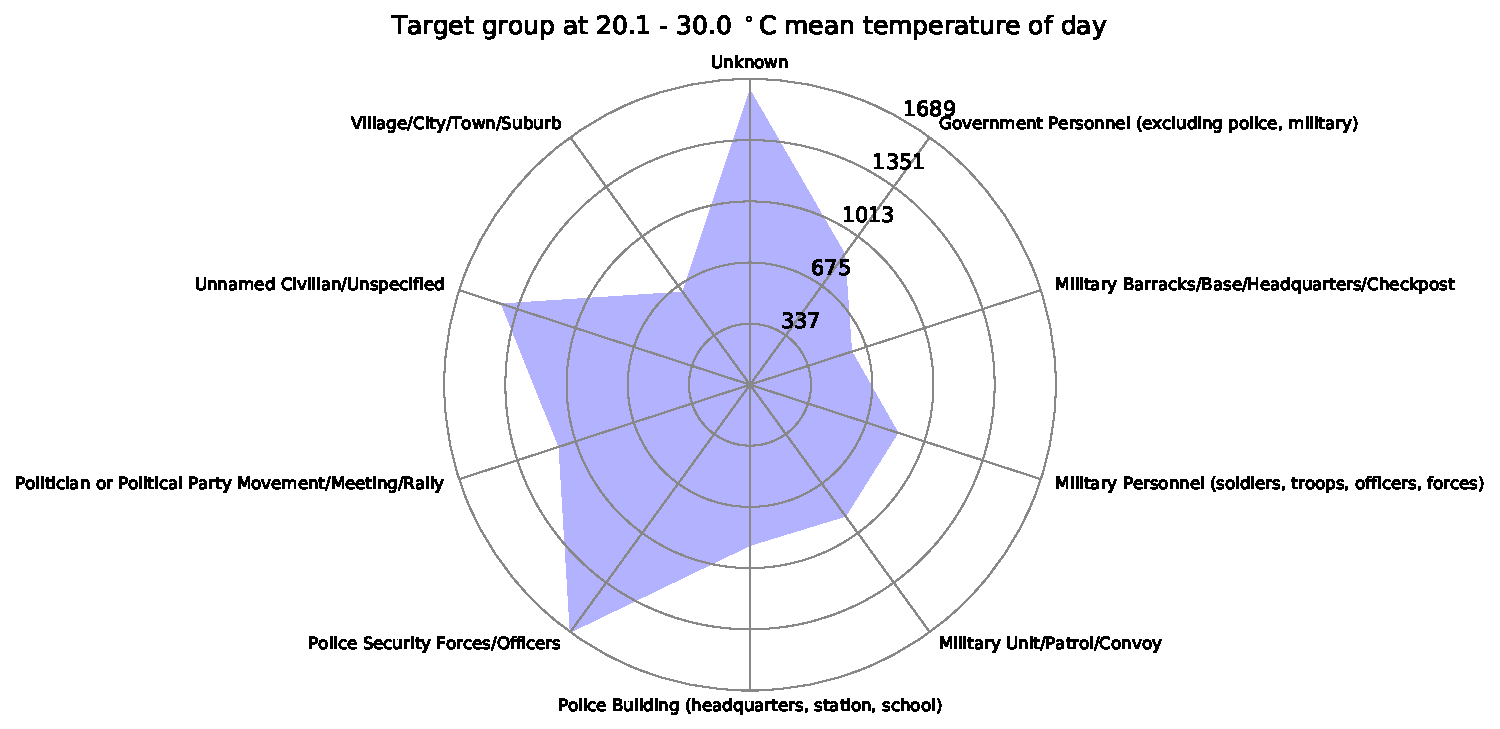
\includegraphics[width=\textwidth]{Temp-Target/temp201-300_starDiagram}
		\end{subfigure}
		\begin{subfigure}[b]{0.3\textwidth}
			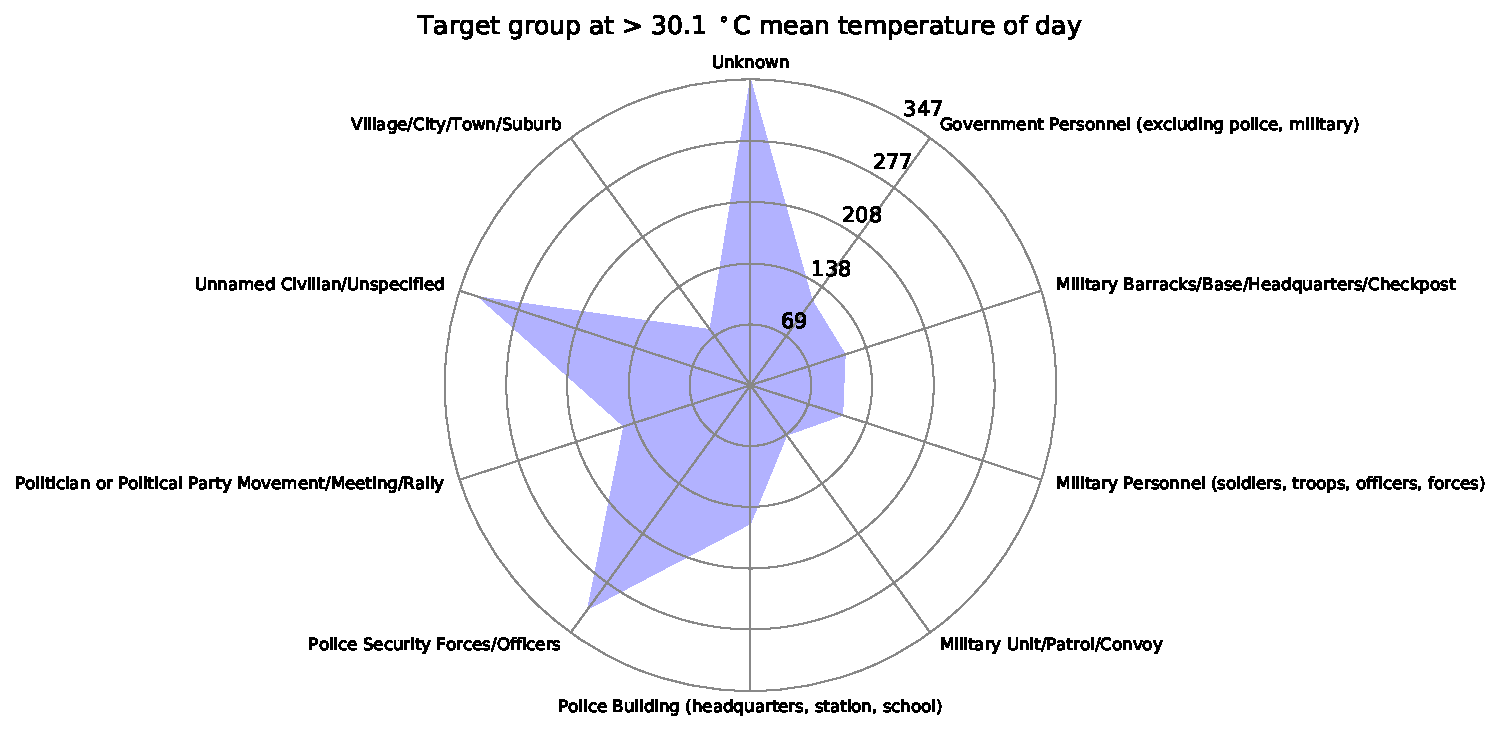
\includegraphics[width=\textwidth]{Temp-Target/temp>301_starDiagram}
		\end{subfigure}
	\end{figure}
	
\end{frame}

\begin{frame}{Results}
	Attack Weapons
	
	\begin{figure}
		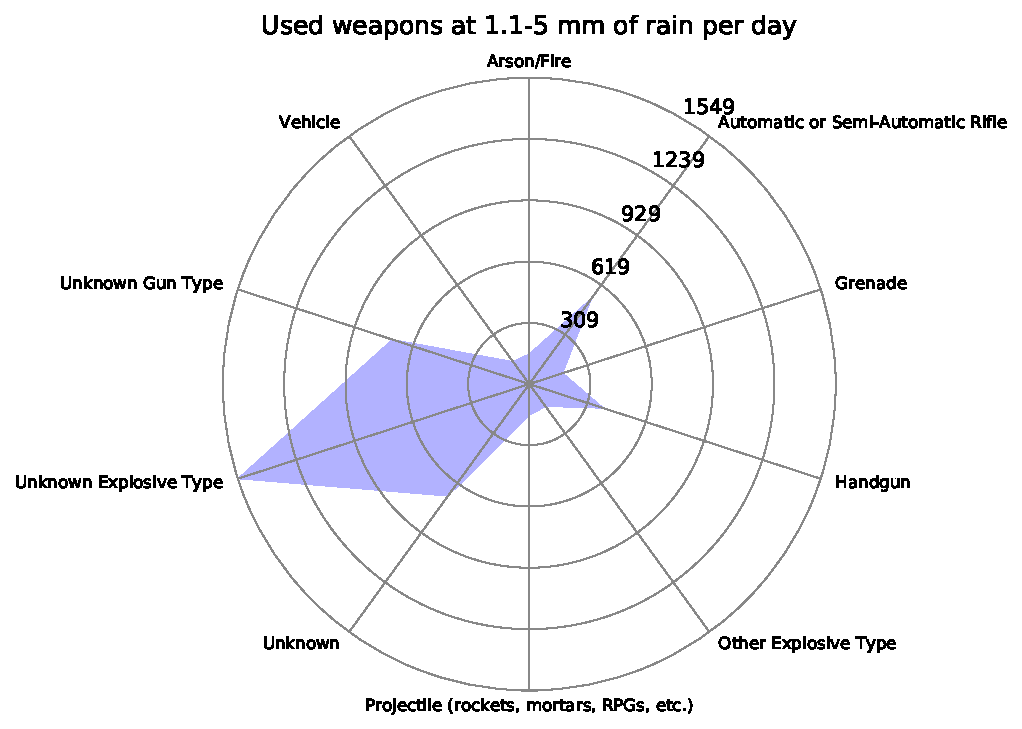
\includegraphics[width=0.8\textwidth]{Rain-Weapon/rain11-5_starDiagram}
	\end{figure}
	
\end{frame}

\begin{frame}{Results}
	\begin{itemize}
		\item 
		Are the used weapons dependent on the weather?
		\begin{itemize}
			\item Attack weapons - Rain
		\end{itemize}
	\end{itemize}
	
	\begin{figure}
		\begin{subfigure}[b]{0.3\textwidth}
			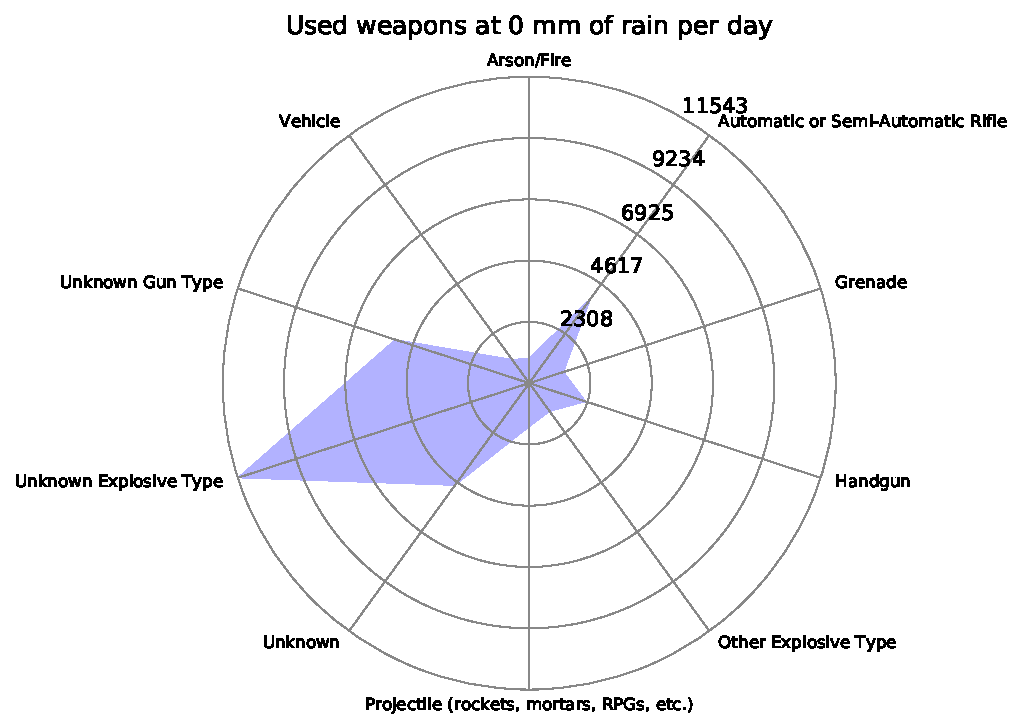
\includegraphics[width=\textwidth]{Rain-Weapon/rain0_starDiagram}
		\end{subfigure}
		\begin{subfigure}[b]{0.3\textwidth}
			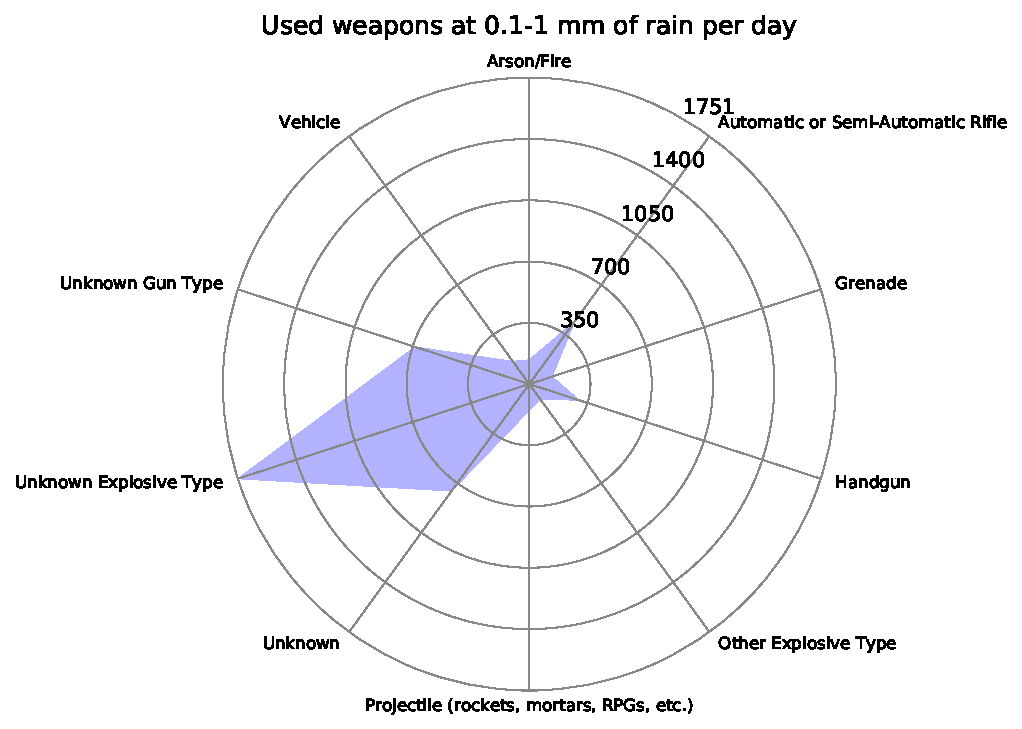
\includegraphics[width=\textwidth]{Rain-Weapon/rain01-1_starDiagram}
		\end{subfigure}
		\begin{subfigure}[b]{0.3\textwidth}
			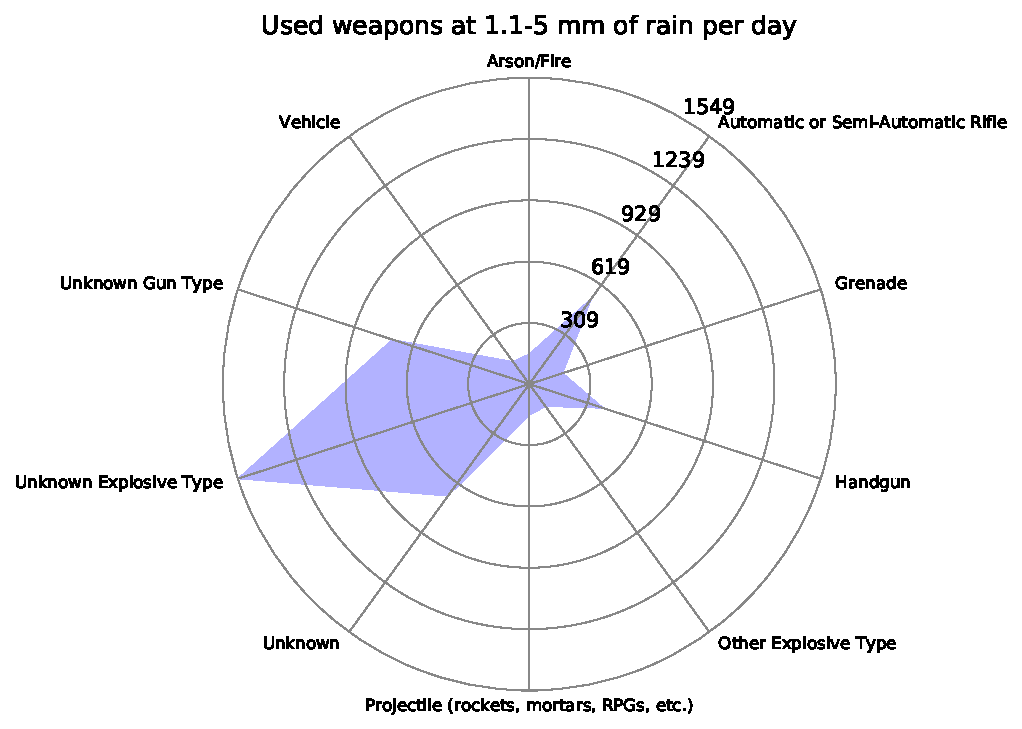
\includegraphics[width=\textwidth]{Rain-Weapon/rain11-5_starDiagram}
		\end{subfigure}
	\end{figure}
	\begin{figure}
		\begin{subfigure}[b]{0.3\textwidth}
			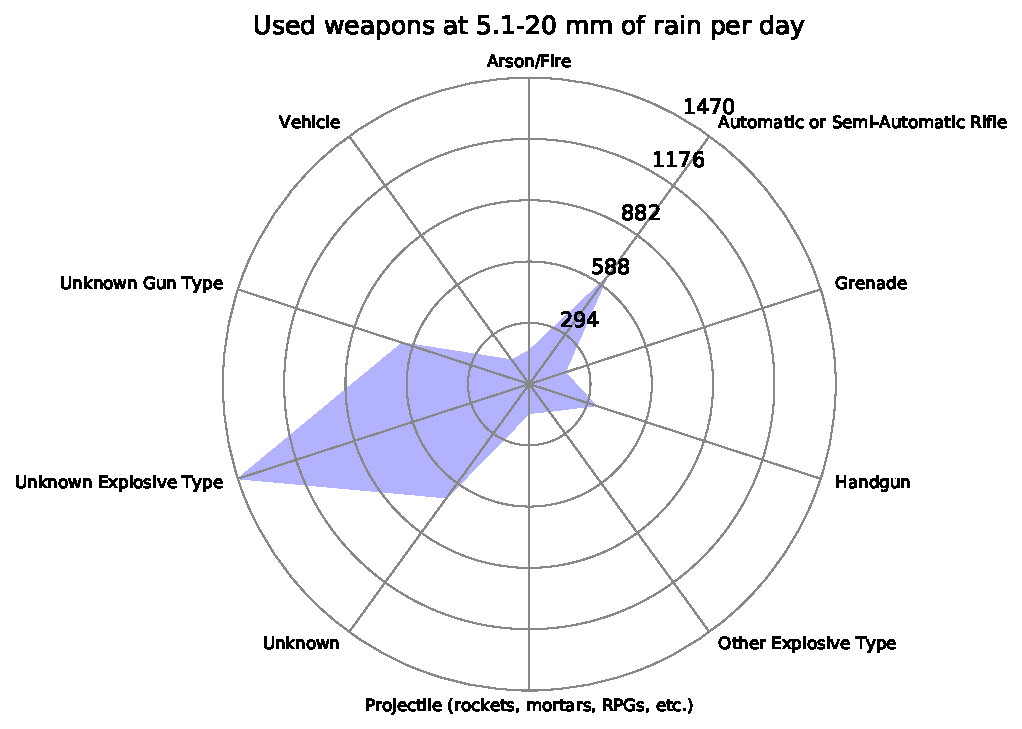
\includegraphics[width=\textwidth]{Rain-Weapon/rain51-20_starDiagram}
		\end{subfigure}
		\begin{subfigure}[b]{0.3\textwidth}
			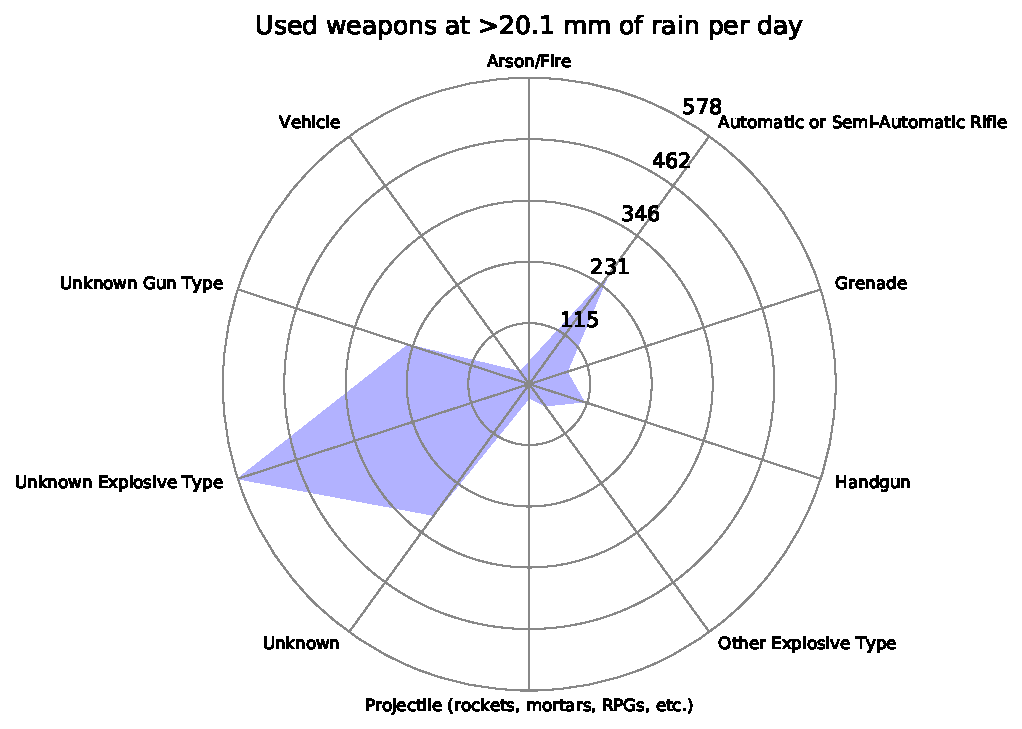
\includegraphics[width=\textwidth]{Rain-Weapon/rain>201_starDiagram}
		\end{subfigure}
	\end{figure}
	
\end{frame}

\begin{frame}{Results}
	\begin{itemize}
		\item 
		Are the used weapons dependent on the weather?
		\begin{itemize}
			\item Attack weapons - Temperature
		\end{itemize}
	\end{itemize}
	
	\begin{figure}

		\begin{subfigure}[b]{0.3\textwidth}
			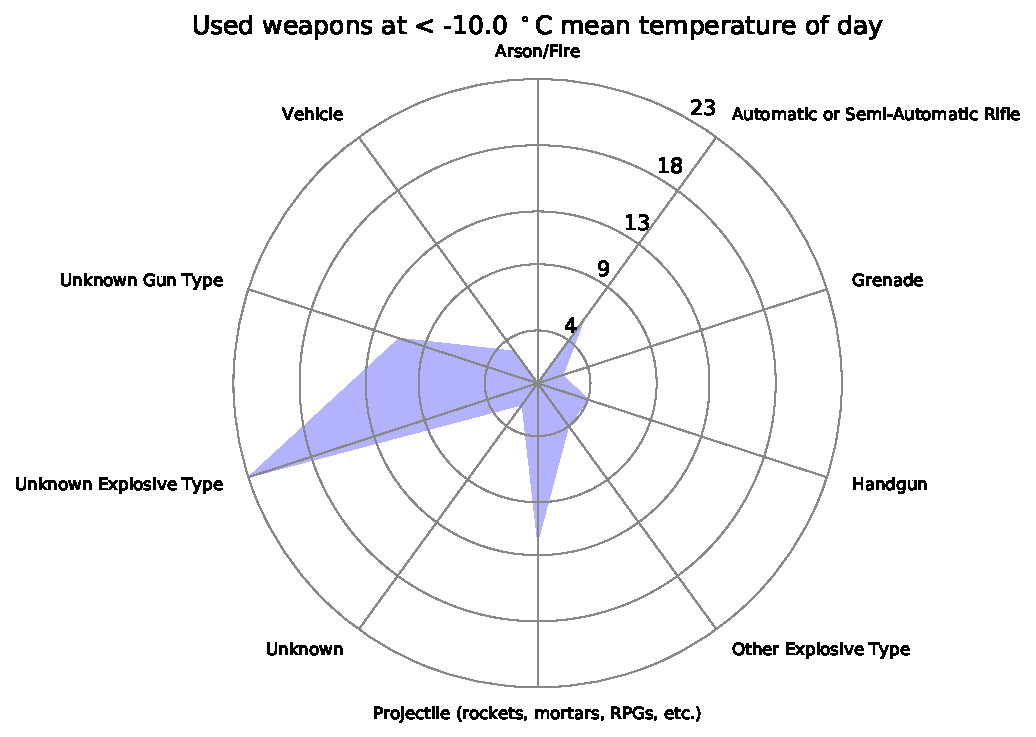
\includegraphics[width=\textwidth]{Temp-Weapon/temp<-100_starDiagram}
		\end{subfigure}
		\begin{subfigure}[b]{0.3\textwidth}
			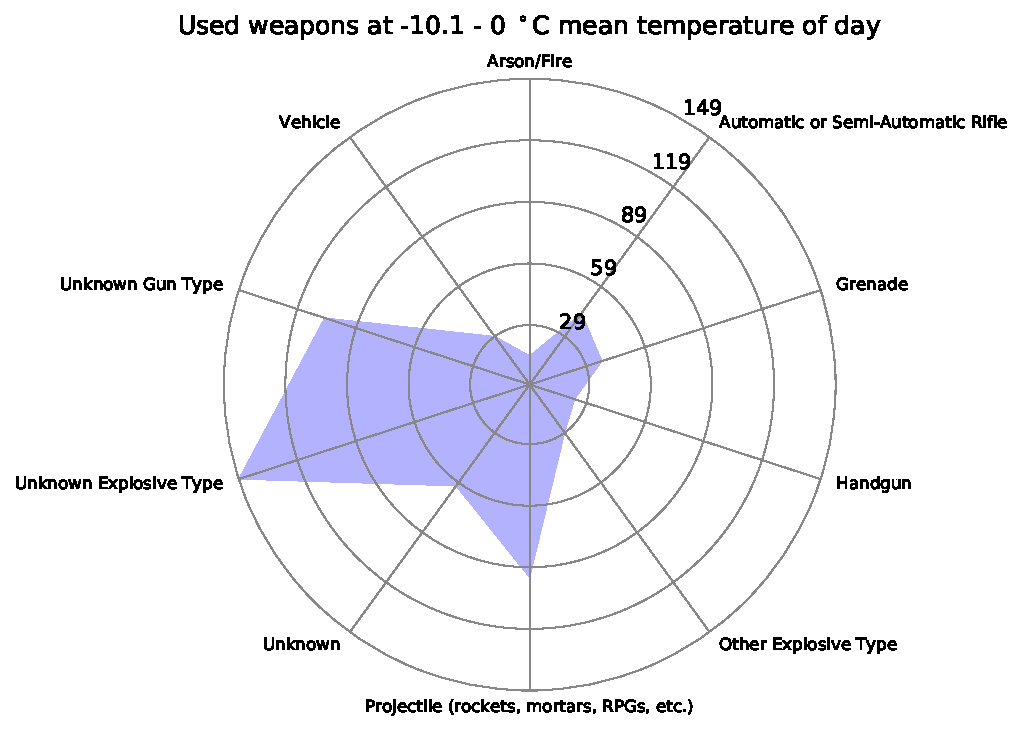
\includegraphics[width=\textwidth]{Temp-Weapon/temp-101-0_starDiagram}
		\end{subfigure}
		\begin{subfigure}[b]{0.3\textwidth}
			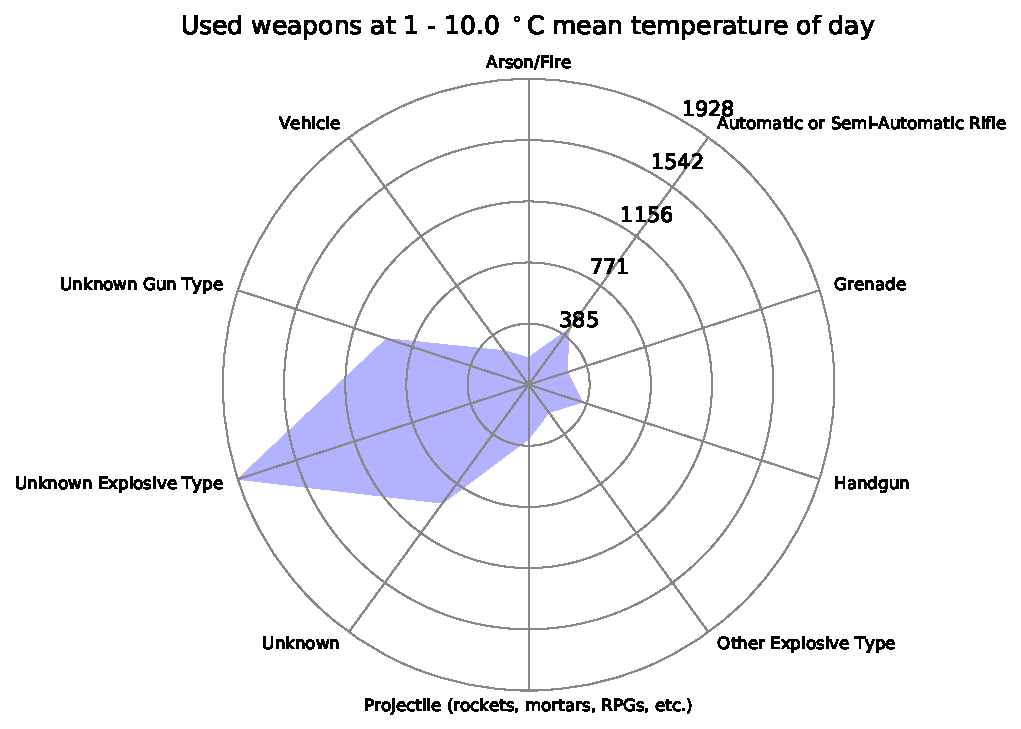
\includegraphics[width=\textwidth]{Temp-Weapon/temp1-100_starDiagram}
		\end{subfigure}
	\end{figure}
	\begin{figure}
		\begin{subfigure}[b]{0.3\textwidth}
			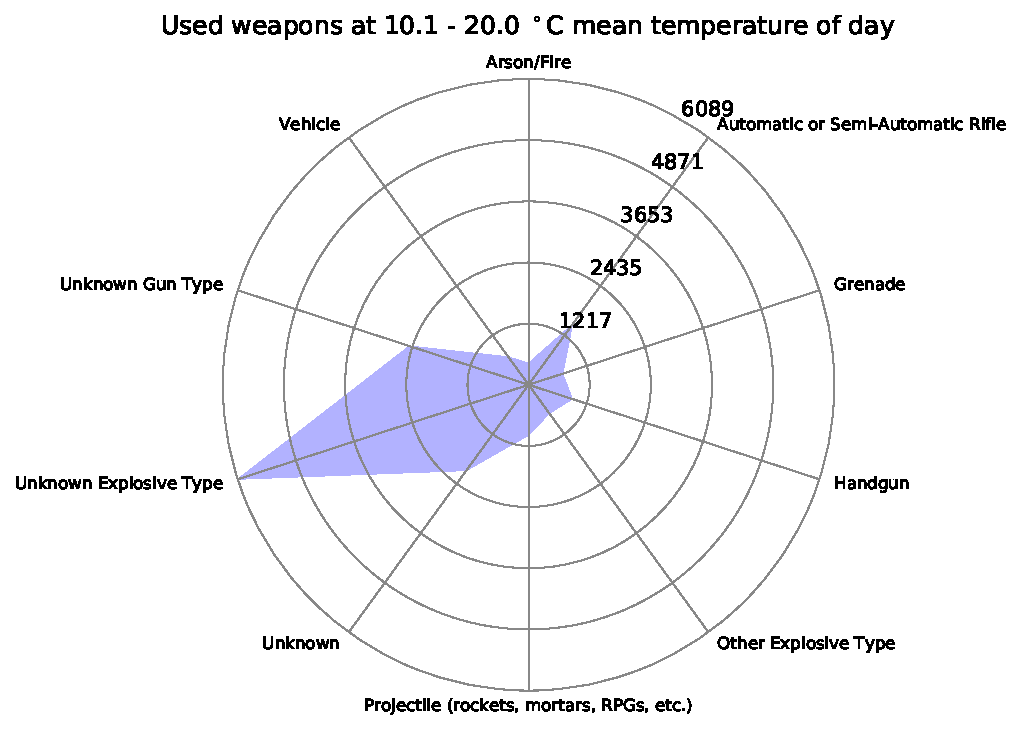
\includegraphics[width=\textwidth]{Temp-Weapon/temp101-200_starDiagram}
		\end{subfigure}
		\begin{subfigure}[b]{0.3\textwidth}
			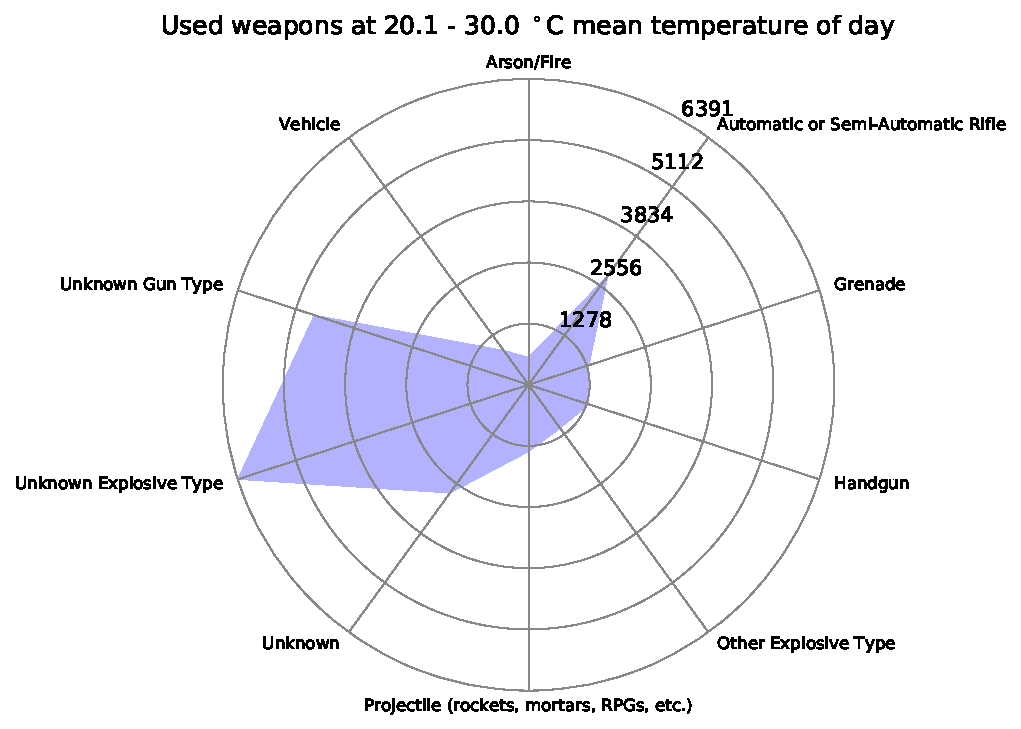
\includegraphics[width=\textwidth]{Temp-Weapon/temp201-300_starDiagram}
		\end{subfigure}
		\begin{subfigure}[b]{0.3\textwidth}
			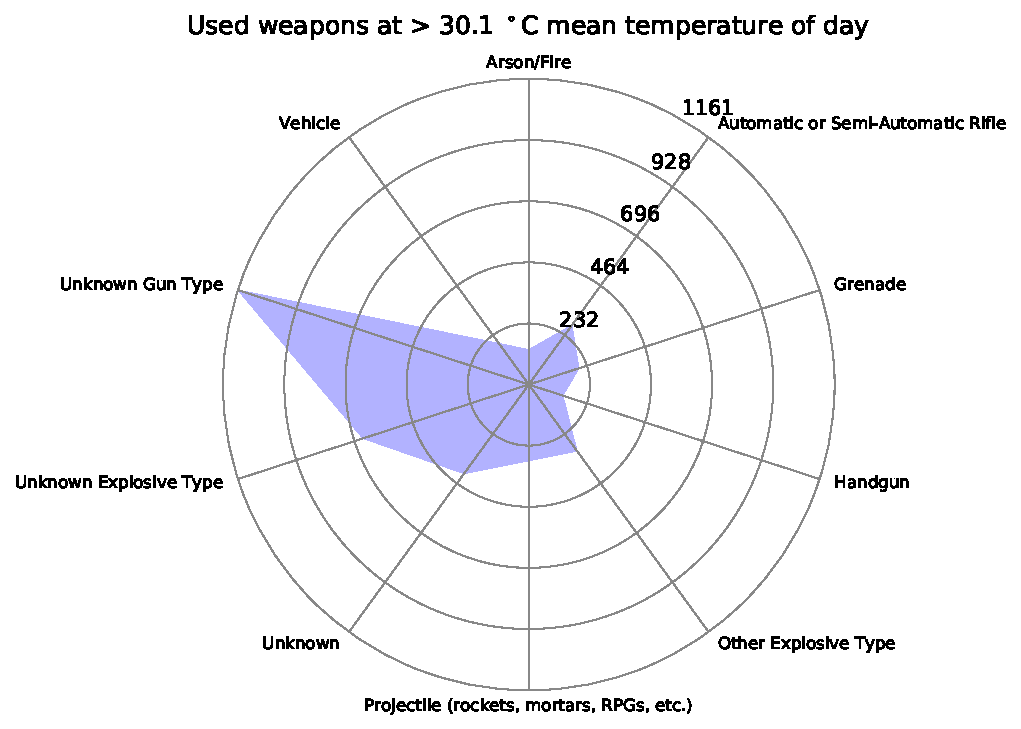
\includegraphics[width=\textwidth]{Temp-Weapon/temp>301_starDiagram}
		\end{subfigure}
	\end{figure}
	
\end{frame}

\begin{frame}{Results}
	Do terror attacks influence founding/splitting of metal bands and vice versa?
	
	\begin{figure}
		\begin{subfigure}[b]{0.3\textwidth}
			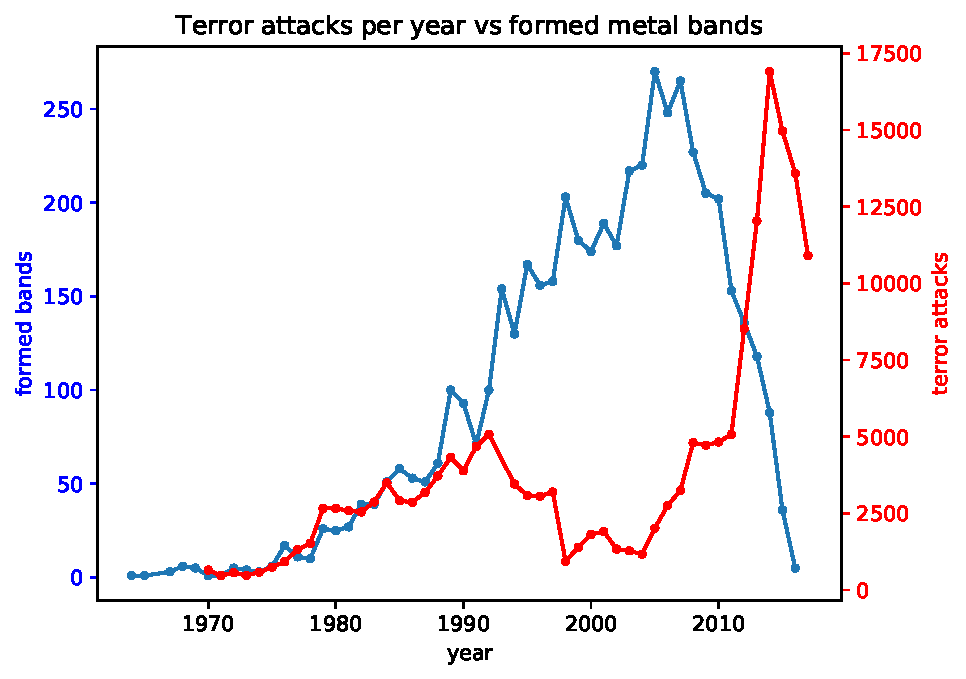
\includegraphics[width=\textwidth]{Band-Terror/attacksVsBandsFormed}
			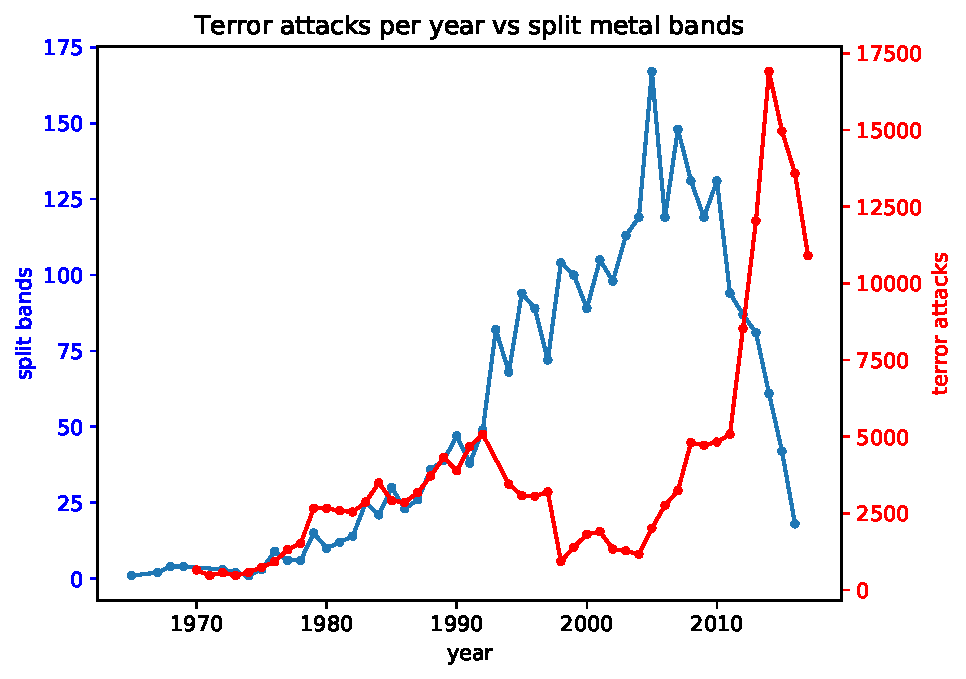
\includegraphics[width=\textwidth]{Band-Terror/attacksVsBandsSplit}
		\end{subfigure}
		\begin{subfigure}[b]{0.65\textwidth}
			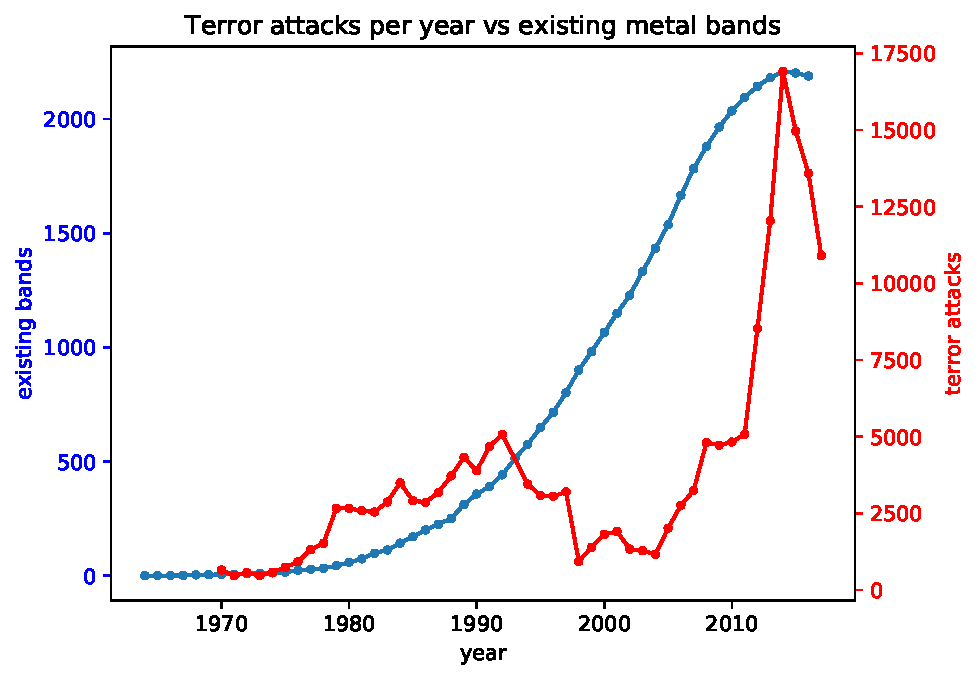
\includegraphics[width=\textwidth]{Band-Terror/attacksVsBandsExisting}
		\end{subfigure}
	\end{figure}
\end{frame}

\begin{frame}{Results}
	Does the population influence the number of existing metal bands?
	
	\begin{figure}
		\begin{subfigure}[b]{0.315\textwidth}
			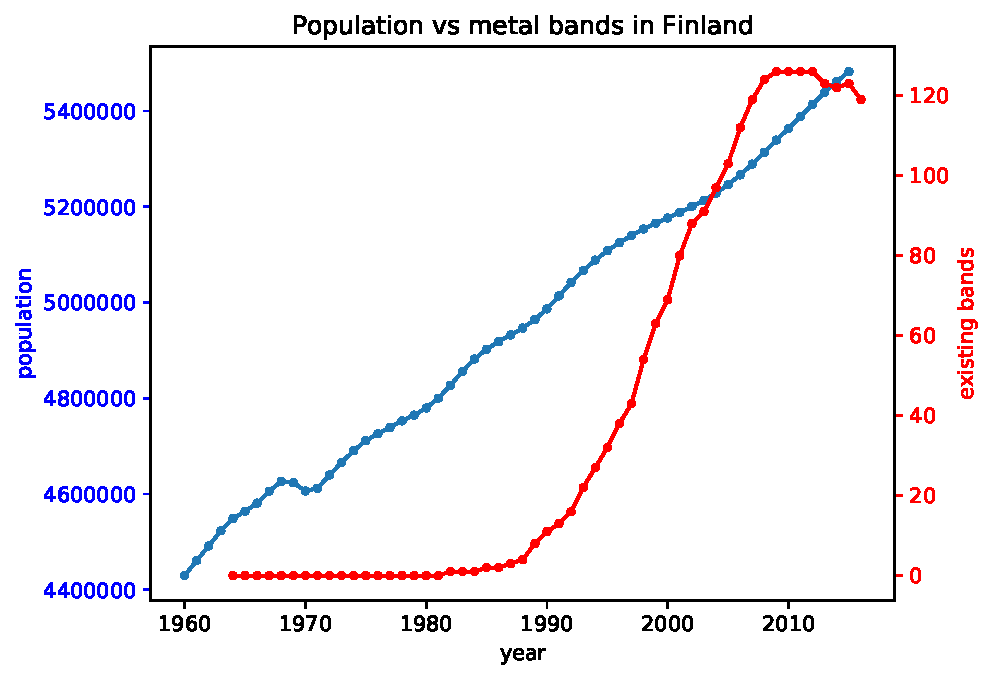
\includegraphics[width=\textwidth]{Population-Bands/populationVsBandFinland}
		\end{subfigure}
		\begin{subfigure}[b]{0.3\textwidth}
			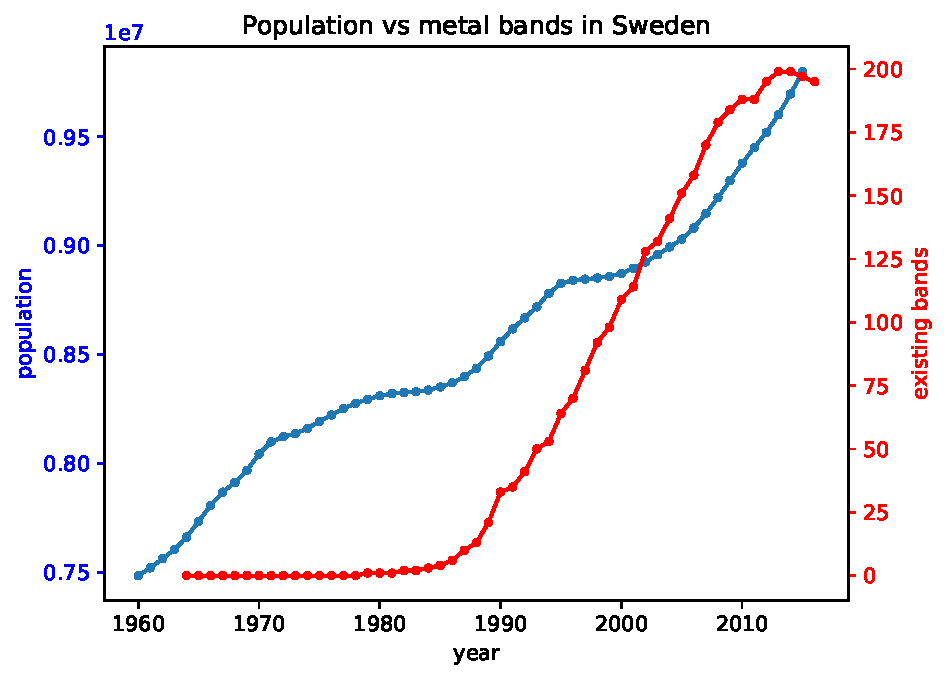
\includegraphics[width=\textwidth]{Population-Bands/populationVsBandSweden}
		\end{subfigure}
		\begin{subfigure}[b]{0.3\textwidth}
			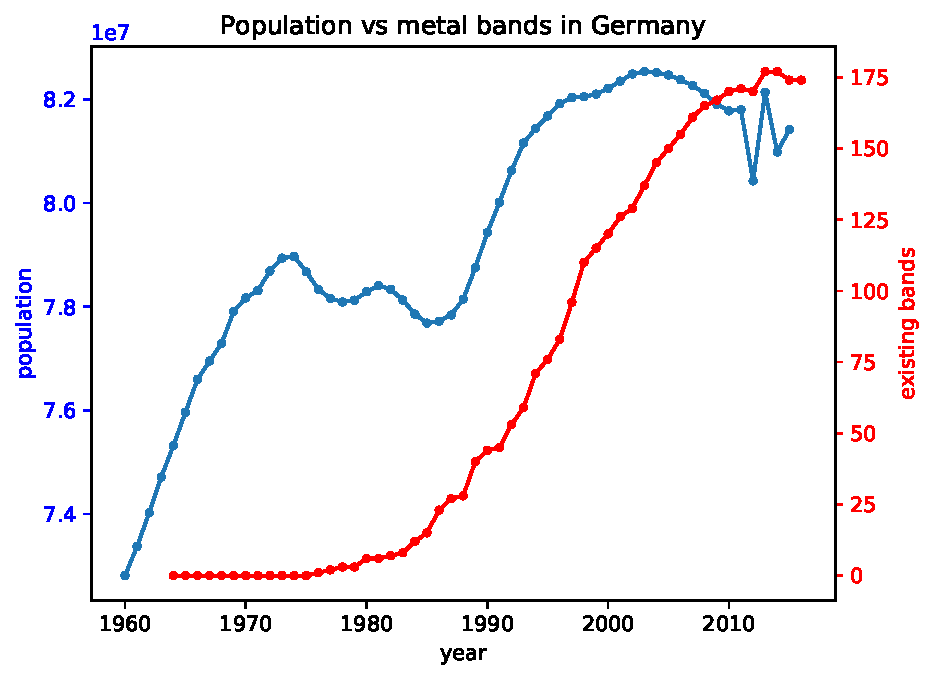
\includegraphics[width=\textwidth]{Population-Bands/populationVsBandGermany}
		\end{subfigure}
	\end{figure}
\end{frame}

\begin{frame}{Results}
	Does the population influence the number of existing metal bands?
	
	\begin{figure}
		\begin{subfigure}[b]{0.315\textwidth}
			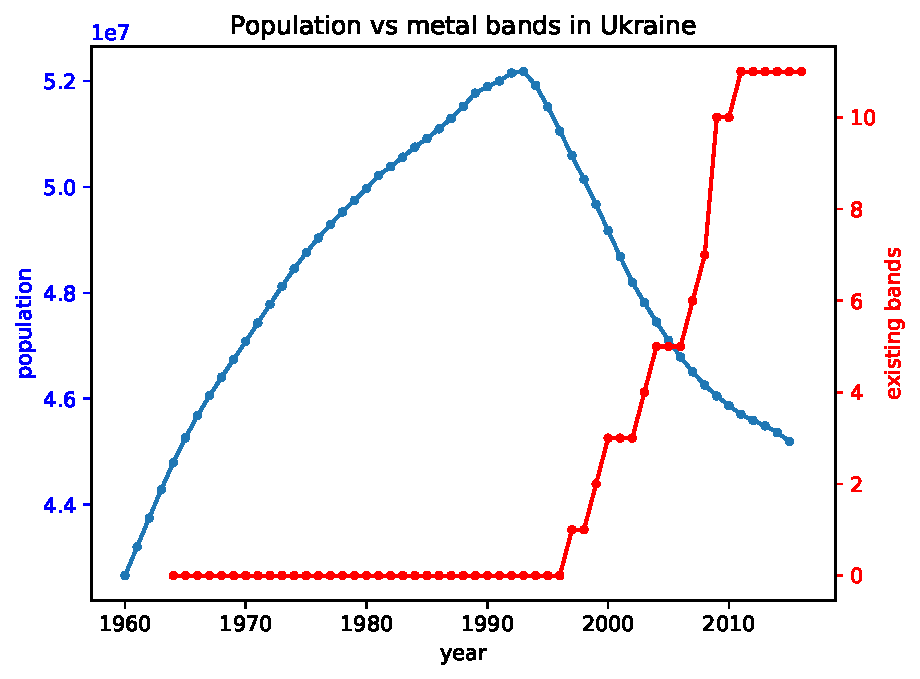
\includegraphics[width=\textwidth]{Population-Bands/populationVsBandUkraine}
		\end{subfigure}
		\begin{subfigure}[b]{0.3\textwidth}
			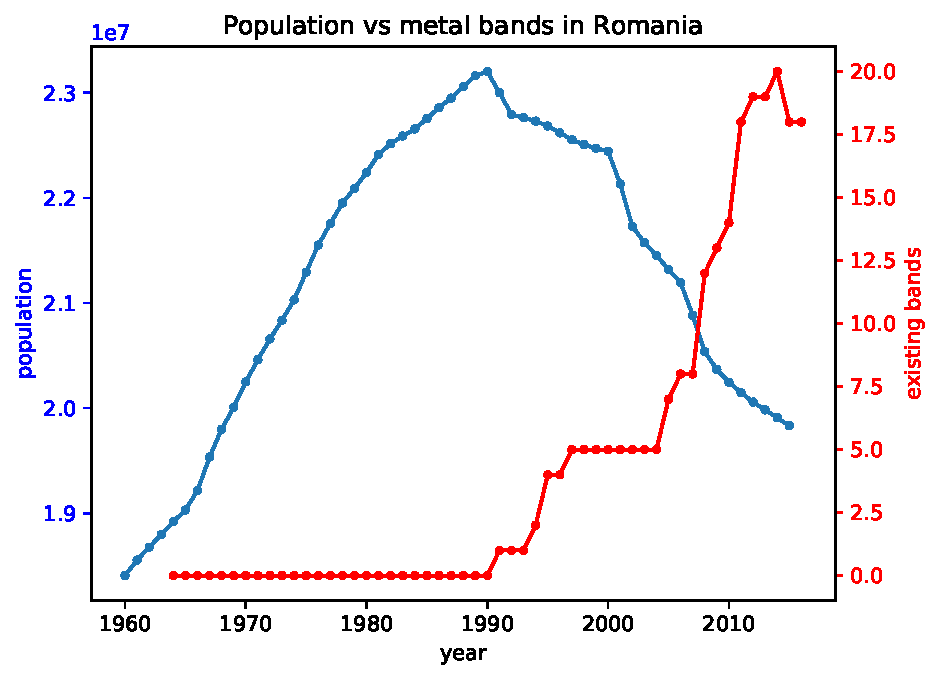
\includegraphics[width=\textwidth]{Population-Bands/populationVsBandRomania}
		\end{subfigure}
		\begin{subfigure}[b]{0.3\textwidth}
			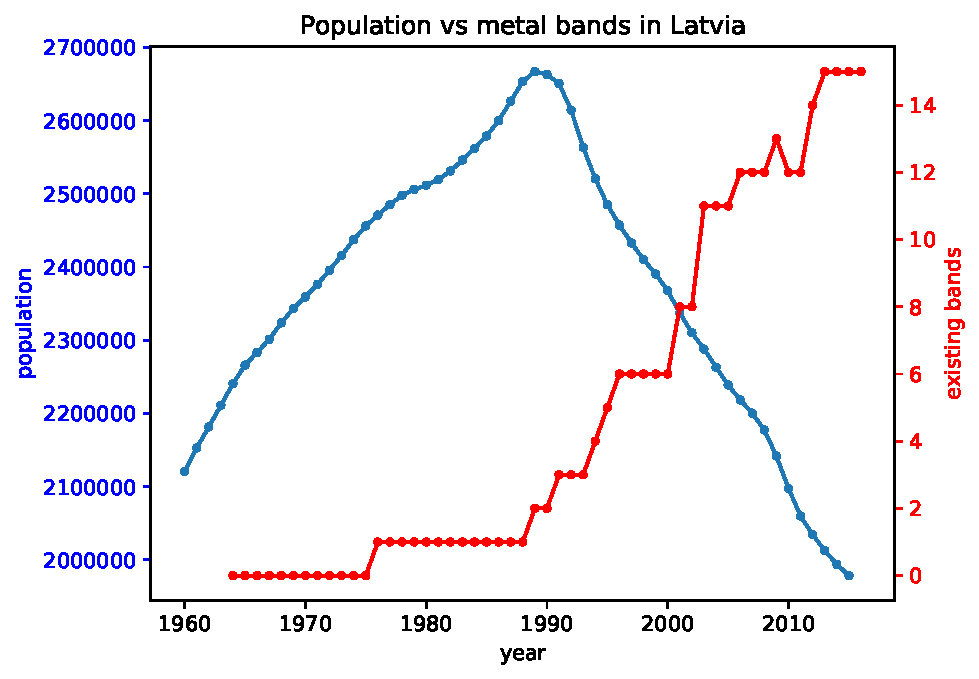
\includegraphics[width=\textwidth]{Population-Bands/populationVsBandLatvia}
		\end{subfigure}
	\end{figure}
\end{frame}

\begin{frame}{Results}
	
	\begin{figure}
		\includegraphics[width=0.8\textwidth]{genreVsTerrorism}
	\end{figure}
	
\end{frame}

\begin{frame}{Results}
	Do terror attacks have an influence on the population?
	
	\begin{figure}
		\begin{subfigure}[b]{0.315\textwidth}
			\includegraphics[width=\textwidth]{Population-Terror/attackVsPopulationSudan}
		\end{subfigure}
		\begin{subfigure}[b]{0.3\textwidth}
			\includegraphics[width=\textwidth]{Population-Terror/attackVsPopulationColombia}
		\end{subfigure}
		\begin{subfigure}[b]{0.3\textwidth}
			\includegraphics[width=\textwidth]{Population-Terror/attackVsPopulationTurkey}
		\end{subfigure}
	\end{figure}
\end{frame}


\begin{frame}{Results}
	Do terror attacks have an influence on the population?
	
	\begin{figure}
		\begin{subfigure}[b]{0.315\textwidth}
			\includegraphics[width=\textwidth]{Population-Terror/attackVsPopulationItaly}
		\end{subfigure}
		\begin{subfigure}[b]{0.3\textwidth}
			\includegraphics[width=\textwidth]{Population-Terror/attackVsPopulationUnitedKingdom}
		\end{subfigure}
		\begin{subfigure}[b]{0.3\textwidth}
			\includegraphics[width=\textwidth]{Population-Terror/attackVsPopulationMoldova}
		\end{subfigure}
	\end{figure}
\end{frame}


% MAP SCREENSHOT
\begin{frame}{Results}
	\begin{figure}
		\begin{subfigure}[b]{\textwidth}
			\includegraphics[width=\textwidth]{911.png}
		\end{subfigure}
	\end{figure}
\end{frame}


% MAP VIDEO
\begin{frame}{Results}
\centering
   \includemovie[
     poster,
     autoplay,
     externalviewer,
     inline=false,
     text={\small(Video)}
   ]{6cm}{6cm}{mapVideo.mp4}
\end{frame}


% QUESTIONS
\begin{frame}
	{\huge Questions?}
\end{frame}


\end{document}

